\documentclass{sig-alternate-05-2015}


\usepackage{amsmath}
\usepackage{listings}
\usepackage{underscore}
\usepackage{enumitem}
\usepackage{etoolbox}
\usepackage{graphicx}
\usepackage{booktabs}
\usepackage{algorithm}
\usepackage{algpseudocode}
\usepackage{pifont}
\usepackage{lipsum,multicol}
\usepackage[T1]{fontenc}
\usepackage{epstopdf}
\epstopdfsetup{outdir=./}
\usepackage{amssymb}
\usepackage{float}
\usepackage{flushend}
\usepackage{caption}


\newcommand{\labac}{$LaBAC_{1}$}
\newcommand{\clabac}{$LaBAC_{0}$}
\newcommand{\hlabac}{$LaBAC_{H}$}
\newcommand{\slabac}{$LaBAC_{S}$}
\newcommand{\consLabac}{$LaBAC_{C}$}

\newcommand{\elabac}{$LaBAC_{E}^{1,1}$}

\newcommand{\clabacOneTwo}{$LaBAC_{0}$}
\newcommand{\hlabacOneTwo}{$LaBAC_{1}$}
\newcommand{\hlabacOneTwoTwo}{$LaBAC_{0}^{2,2}$}
\newcommand{\labacZeroTwoTwo}{$LaBAC_{0}^{2,2}$}
\newcommand{\labacOneOneOne}{$LaBAC_{1}$}
\newcommand{\labacZeroOneOne}{$LaBAC_{0}$}
\newcommand{\labacZeroMN}{$LaBAC_{0}^{m,n}$}
\newcommand{\abacAlpha}{ABAC_\alpha}
\newcommand{\hgabac}{HGABAC}
\newcommand{\uLabel}{uLabel}
\newcommand{\oLabel}{oLabel}

\newcommand{\uLabelOne}{uLabel_1}
\newcommand{\oLabelOne}{oLabel_1}
\newcommand{\uLabelTwo}{uLabel_2}
\newcommand{\oLabelTwo}{oLabel_2}
\newcommand{\canAddPolicy}{can\_manage\_policy}



%-- LaBAC new commands---

\newcommand{\lb}{ }
\newcommand{\OBJ}{O}
\newcommand{\objmem}{o}
\newcommand{\U}{U}
\newcommand{\umem}{u}
\newcommand{\amem}{a}
\newcommand{\A}{A}
\newcommand{\OL}{OL}
\newcommand{\UL}{UL}
\newcommand{\OLV}{OL}
\newcommand{\olvmem}{ol}
\newcommand{\ULV}{UL}
\newcommand{\ulvmem}{ul}
\newcommand{\OLA}{OLA}
\newcommand{\ULA}{ULA}
\newcommand{\OLH}{OLH}
\newcommand{\ULH}{ULH}

\newcommand{\Policy}{Policy}
\newcommand{\policy}{Policy}

\newcommand{\creator}{creator}

\newcommand{\odominate}{\succeq_{ol}}
\newcommand{\udominate}{\succeq_{ul}}

\newcommand{\allowedLabels}{allowed\_counter\_labels}
\newcommand{\restrictedTuples}{RestrictedTuples}



\newcommand{\oLabelH}{oLabel^*}
\newcommand{\uLabelH}{uLabel^*}
\newcommand{\impliedPolicy}{ImpliedPolicy}
\newcommand{\effectivePolicy}{Effective\_policy}
\newcommand{\policyBound}{ValidTuples}
\newcommand{\sessionLabels}{s\_labels}
\newcommand{\CircuitSAT}{CircuitSAT}
\newcommand{\maxPolicy}{|policy|_{max}}
\newcommand{\maxPolicySet}{|\policy|_{max}}
\newcommand{\request}{is\_authorized}



\newcommand{\requestContext}{ReqContext}
\newcommand{\reviewFunction}{R}

\newcommand{\sABAC}{$ABAC_s$}

\newcommand{\twoSortedRBAC}{2-sorted-RBAC}
\newcommand{\properRole}{R^+}
\newcommand{\properRoleHierarchy}{R^+H}
\newcommand{\demarcationHierarchy}{D^+H}
\newcommand{\roles}{R^+}
\newcommand{\RH}{R^+H}
\newcommand{\demarcation}{D^+}
\newcommand{\DeH}{D^+H}
\newcommand{\PD}{PD^+}
\newcommand{\SR}{SR^+}

%----------------Session / object creation functions--------------%
\newcommand{\createSession}{create\_session}
\newcommand{\deleteSession}{delete\_session}
\newcommand{\assignValues}{assign\_values}
\newcommand{\removeValues}{remove\_values}
\newcommand{\createReq}{session^+}
\newcommand{\removeReq}{session^-}
\newcommand{\sessionOL}{session}
\newcommand{\createObject}{create\_object}
\newcommand{\updateObject}{update\_OL\_values}
\newcommand{\assignLabels}{assign\_OL\_values}
\newcommand{\removeLabels}{remove\_OL\_values}

\newcommand{\createUser}{create\_user}
\newcommand{\assignULLabels}{assign\_UL\_values}
\newcommand{\removeULLabels}{remove\_UL\_values}

%-------------Policy Machine Command--------------------%
\newcommand{\pmMini}{PM_{mini}}
\newcommand{\assignment}{ASSIGN}
\newcommand{\assignmentPlus}{\assignment^+}
\newcommand{\assignmentStar}{\assignment^*}
\newcommand{\assignmentOOA}{\assignment_{ooa}}
\newcommand{\assignmentUUA}{\assignment_{uua}}
\newcommand{\assignmentOAOA}{\assignment_{oaoa}}
\newcommand{\assignmentUAUA}{\assignment_{uaua}}
\newcommand{\assignmentATPC}{\assignment_{atpc}}
\newcommand{\association}{ASSOCIATION}
\newcommand{\associationPolicy}{\association_{policy}}
\newcommand{\decisionFunction}{allow\_resource\_request}
\newcommand{\allAssignment}{ASSIGN}
\newcommand{\allAssociation}{ASSOC}
\newcommand{\peAssoc}{PC\_ASSOC}
\newcommand{\peAssign}{PC\_ASSIGN}
\newcommand{\assignmentLabac}{\assignment}


%\pagenumbering{arabic}

%\documentclass{article}
\begin{document}
\title{Label-Based Access Control: An ABAC Model \\with Enumerated Authorization Policy}


 \numberofauthors{3}
\author{
\alignauthor Prosunjit Biswas\\
       \affaddr{Univ. of Texas at San Antonio}\\
       \email{eft434@my.utsa.edu }
\alignauthor Ravi Sandhu\\
	\affaddr{Univ. of Texas at San Antonio}\\
	\email{ravi.sandhu@utsa.edu}
\alignauthor Ram Krishnan\\
	\affaddr{Univ. of Texas at San Antonio}\\
	\email{ram.krishnan@utsa.edu }
}

\date{30 July 1999}

\CopyrightYear{2016}
\setcopyright{acmcopyright}
\conferenceinfo{ABAC'16,}{March 11 2016, New Orleans, LA, USA}
\isbn{978-1-4503-4079-3/16/03}\acmPrice{\$15.00}
\doi{http://dx.doi.org/10.1145/2875491.2875498}

\maketitle




\begin{abstract}
	
 There has been considerable research in specifying authorization policies for XML documents. Most of these approaches consider only \textit{hierarchical structure} of underlying data. They define authorization policies by directly identifying XML nodes in the policies. These approaches work well for hierarchical structure but are not suitable for other required characteristics we identify in this paper as \textit{semantical association} and \textit{scatteredness}.
 
 
This paper presents an attribute based protection model for JSON documents. We assign \textit{security-label} attribute values  to JSON elements and specify authorization policies using these values. By using security-label attribute, we leverage  semantical association and scatteredness properties. Our protection mechanism defines two types of policies called  authorization and labeling policies. We present an operational model to specify authorization policies and  different models for defining labeling policies. Finally, we demonstrate a proof-of-concept for the proposed models in the Swift service of OpenStack IaaS cloud.

% In our approach, we assign \textit{security-label} attribute values  to JSON elements in a JSON document and specify authorization policies using these attribute values. Thus, our protection model have a  level of indirection where JSON objects are first annotated with security-label values which can  be managed independently from the JSON documents and seamlessly with other higher level organizational policies. We lay out an architecture of our protection model and  specify labeling policies to assign attribute values to JSON objects. Our protection model is significantly different than most of the existing XML protection models which directly assign authorization policies on XML nodes. These models (XML models) may result duplicated authorization policies which are hard to manage or administer. We believe, our protection model can also be used for XML data as well.


% and Our protection model is significantly different than most of the existing XML protection models which could have been  adopted for protecting JSON documents. In this perspective, we argue that most of the existing protection models for XML directly assign authorization policies on XML nodes which leaves the possibility of duplicated authorization policies for similar (in term of authorization requirement) but different information. 


 %While XML and JSON 
	
%JSON or JavaScript Object Notation is an open standard for data interchange which is gaining immense popularity due to its concise representation and ease of human and machine readability. Industries are increasingly adopting JSON for internal data representation and data transfer format which is reflected by developments including JSON  document database such as MongoDB (more accurately BSON, a modified version JSON) is now officially supported by the OpenStack cloud platform, Twitter latest API (v 1.1) supports only JSON and YouTube latest API (v 3) recommends JSON as the default exchange format. Interestingly, in spite of industry demand, JSON has received minimal interest from the research community.

%In this paper, we investigate access control scope for JSON documents. We present a label based protection mechanism for JSON data. For this purpose, we have demonstrated a simple label based access control model and shown different ways (path based, content based and attribute based) of labeling JSON items automatically or semi-automatically to reduce labeling efforts. We have also specified label based constraints to capture practical labeling requirements. We have implemented the protection mechanism for JSON documents stored as OpenStack Swift objects. As part of our implementation, we have extended ACL based `all or nothing' access of a Swift object towards content level partial access.

%We present a simple attribute based access control model for this purpose and demonstrate a corresponding protection mechanism.  To the best of our knowledge, we are the first to attempt this kind of work for JSON documents. We have implemented  our proposed access control model and made it available as a standard package in the official Python repository.
\end{abstract} 

\chapter{Introduction}






\section{Motivation}




\section{Problem statement and thesis}
\subsection{Problem statement}
There are two major techniques for specifying authorization policies in Attribute Based Access Control (ABAC). The more conventional approach is to define policies using logical formulas involving attribute values. The alternate technique is by enumeration. While considerable work has been done for the former approach, the later  lacks fundamental work from the research community.

\subsection{Thesis}
\textit{Enumerated Authorization Policy ABAC (EAP-ABAC) model is a viable alternate to Logical-formula Authorization Policy ABAC (LAP-ABAC) model. EAP-ABAC is as expressive as LAP-ABAC in the finite domain. EAP-ABAC models can be enforced in different application domains.}


\section{Summary of contribution}

\section{Organization of the dissertation}


%\section{Administrative Reviews in ABAC}
Administrative review functions or simply review functions of an access control model provides capability to pose queries on basic sets (e.g. users, object), elements (e.g. attributes) and relations (user-role assignment, user-attribute assignment) of the model. For example, review functions in RBAC \cite{nist-rbac} ask for roles assigned to a user, or users assigned to a role and so on. These capabilities allow an administrator to audit or troubleshot  a system, update existing policies and/or define more precise policies. For example, before assign a new role to a user, it may be desirable to see first what roles the user already posses. 

Like review functions play an important role in RBAC model (30+ review function being defined in NIST RBAC model), there are significant needs for review facilities in the context of ABAC model. For example, before assigning a new value to an  attribute (say, `clearance') of a user, it is desirable to see what `clearance' values the user has already been assigned. Similarly, administrators may want to see, with the available clearances what permissions the user has authority to exercise. A careful administrator would also want to check, what additional permission the user gains with assignment of a new clearance value. 

	\begin{figure} 
		\centering
		\includegraphics[width=.4\textwidth]{review-function-diagram}
		\caption{Review functions in ABAC}
		\label{fig:labac}
	\end{figure}
	

% Please add the following required packages to your document preamble:
% \usepackage{booktabs}
\begin{table}
	\centering
	\caption{Some review questions on an ABAC model} %\vspace*{3pt}
	\label{tab:review-functions-example}
	\begin{tabular}{|l|}						
		\hline					
		\multicolumn{1}{|c|}{\underline{\textit{I. Attribute Reviews }}}\\				 
		
			 1. What attributes are assigned to a user? \\
			 2. What are the values of a user attribute for a given user? \\
			 3. Which users are assigned to a given (attribute, value) pair? \\
			 4. Values of an object attribute? \\
			 5. What objects are assigned to a (attribute,value) pair ? \\
			 
		\multicolumn{1}{|c|}{\underline{\textit{II. Permission Reviews}}} \\		
		
	     	1. What permissions a user has? \\
	     	2. What permissions a user gains or looses after being assigned  \\ \hfil to a new attribute value? \\	     	 
	     	3. For a  certain permission, which attribute, values are required? \\
	     	
		\multicolumn{1}{|c|}{\underline{\textit{III. Policy Reviews}}} \\
		
			 1. Which users are allowed by a given policy? \\
			 2. Which objects are allowed by a given policy? \\
			 3. Which actions are granted by a given policy?\\
			 4. Which users (in term of (attribute, value) pair) are granted \\ \hfil what actions  on which objects (in term of (attribute, value) pair)?
		\\ \hline	
	\end{tabular}	
\end{table}


In addition to reviews on attributes, we can also pose interesting review questions on policies. While, some review questions may need to consider all  available policies in the system, some other simple reviews can be answered using a candidate policy. For simplicity, in this section, we are interested only on those simple review functions. Informally, let us assume an ABAC policy that says `users with clearance manager can approve existing loan' for user attribute `clearance' and value from the set \{manager, employee\}, object attribute `loan' and value from the set  \{existing, default\} and  and action 'approve'. Some simple review questions that we can ask using this policy include - a. who can approve existing loans ? b. which type of loan a manager can approve? c. who can approve which loans so on.

To formally define review functions, in the following section we first define a simple ABAC model - \sABAC{}. We follow the conventional approach for designing policies based on flexible policy language. In Section \ref{sec:review-function}, we define review functions using the \sABAC{} model. In Section \ref{section:np-complete}, we show that even simple policy review in \sABAC{} is NP-Complete. 

	
\newcommand{\phiu}{\phi_{u}}
\newcommand{\phio}{\phi_{o}}
\newcommand{\phia}{\phi_{a}}
\newcommand{\phip}{\phi_{p}}
\newcommand{\phix}{\phi_{x}}
\newcommand{\phiy}{\phi_{y}}
\newcommand{\userAttrExpr}{UAExpr}
\newcommand{\objectAttrExpr}{OAExpr}
\newcommand{\actionExpr}{AExpr}
\newcommand{\review}{acting\_users}
\newcommand{\simpleReview}{deep\_review}
\newcommand{\isSatisfiable}{is\_satisfiable}
\newcommand{\interpretationY}{I_y}
\newcommand{\interpretationX}{I_x}
\newcommand{\interpretation}{I}
\newcommand{\reductionAlgo}{CircuitSAT2PolicyReview}
\newcommand{\psiu}{\psi_{u}}



\subsection{\sABAC{} as a Conventional ABAC Model}
\sABAC{} model is defined for a finite set of users $U$, objects $O$ and actions $A$. Additionally, it has a set of attribute functions for users and objects. One or more user attributes form UAExpr, one of more object attributes form OAExpr and oen or more actions from AExpr.

	
\newcommand{\policyEval}{\delta}
% Please add the following required packages to your document preamble:
% \usepackage{booktabs}
\begin{table*}
	\centering
	\caption{  \sABAC{} Model} %\vspace*{3pt}
	\label{tab:labac-definition}
	\begin{tabular}{|l|}						
		\hline					
		\multicolumn{1}{|c|}{\underline{\textit{I. \sABAC{} Model } } }\\	
		
	 	- $U, O, A$: set of users, objects and actions \\
	 	- $UA,OA$: set of attribute functions for users and objects respectively.   \\ \hfill	$for_{ua \in UA}, ua: U \to 2^{range(ua)} $ and
	 	$for_{oa \in UA}, oa: O \to 2^{range(oa)} $ \\
	 	- policy: for an action, a policy $\phi_a$ is defined as shown in table \ref{tab:sabac-def}\\
	 	%-  policy: For an action a, a policy \phi_a is defined as shown table ?? \\
	 	 
	 
	 \hline	
	\end{tabular}
	
\end{table*}

%mod

	\newcommand{\UAttrVal}{\text{UAttrVal}}
\newcommand{\OAttrVal}{\text{OAttrVal}}
\newcommand{\Action}{action}
\newcommand{\E}{E}
% Please add the following required packages to your document preamble:
% \usepackage{booktabs}
\begin{table}[]
\centering
\caption{Policy Definition for \sABAC}
\label{tab:sabac-def}
\begin{tabular}{@{}l@{}}
 \hline
	$\phi ::= \phi \land \phi | \ \phi \lor \phi | \ (\phi) | \neg \phi $\\
 
	$\phi ::= \E $ \\
	Terminal Symbols:\\
	$ \E (attr: UA \cup OA, val: range(Attr))$ \\ \hfill  $\to \{true, false\}$ \\
	%$Act(\requestContext, a) \to \{true, false\}$\\
 %\bottomrule
 \\\hline
\end{tabular}
\end{table}

 
	


\subsection{Review Functions in \sABAC{}}
	

\textbf{Interpretation of Attribute Expression}\\
	Informally, an interpretation of an attribute expression  is the set of  $(attr,Value)$ pairs where $attr \in UA \cup OA$ and $Value \subseteq Range(attr)$ for which the attribute expression is evaluated to be true. Formally, we define interpretation as a function $\interpretation$ as follows.

\begin{itemize}
	\item $\interpretation(\phi) \to 2^{(attr: UA \cup OA,  Value: 2^{Range(attr)})}$ and  defined as \\
	$\interpretation(\phi) = \{(attr,Value) | (E(attr,val) \implies true ) \implies (\phi \implies true) \land val \in Value \}$
	
\end{itemize}
	
\noindent \textbf{Example of \sABAC{} Policy and its interpretation} \\
let $ \phi  \equiv \{ E(role, manager) \land \lnot E(role, dir) \land E(type, new) \}$ be a  \sABAC  policy. 	
$I_\phi = \{ (role,  \{ manager\}),$  $(type, \{ new\}), $   $(action, \{ approve\}) \}$ is satisfying interpretation for $\phi $. but $\{ (role,  \{ manager, dir\}) , (type, \{ new\}),$ \\ $(action, \{ approve\}) \}$ is not a satisfying interpretation. \\

\noindent \textbf{Review Function As a Decision Problem}
	
$\simpleReview=\{  \phi$ | exists an assignment of user and object attribute values of policy $\phi$ st. $\phi$ is evaluated true \}  \\
	
%Finally, we define review function $\reviewFunction$ as follows.$R(\phi, input:2^{\interpretation_\phi}) \to 2 ^{\interpretation_\phi}$, defined as  $R(\phi, input) = 2^{\interpretation_\phi} \setminus input$ \\	\\



 
 
% % Please add the following required packages to your document preamble:
 % \usepackage{booktabs}
 \begin{table}
 	\centering
 	\caption{Some review functions for \sABAC{}}
 	\label{tab:review-fun}
 	\begin{tabular}{|l|l|l|}
 		 \hline
 		 \textit{function Name} &  \textit{Input} &  \textit{Output}\\
 		 \hline
 		 \textit{\request} &   \{$\interpretation(\phiu), \interpretation(\phio), \interpretation(\phia)$\}&  $\delta \equiv \{true, false\}$ \\ 		 
 		 
 		 \hline
 		 \textit{UA-query} &   \{$ \interpretation(\phio), \interpretation(\phia), \delta$\}&  $\{\interpretation(\phiu)\}$ \\
		\hline
		\textit{OA-query} &   \{$ \interpretation(\phiu), \interpretation(\phia), \delta$\}&  $\{\interpretation(\phio)\}$ \\
		\hline
		\textit{Act-query} &   \{$ \interpretation(\phiu), \interpretation(\phio), \delta$\}&  $ \{ \interpretation(\phia) \}$ \\
		\hline
		\textit{UO-query} &   \{$ \interpretation(\phia), \delta$\}&  $ \{ \interpretation(\phiu),\interpretation(\phio) \}$ \\
			\hline
		\textit{deep-query} &   \{$\delta$\}&  $ \{ \interpretation(\phiu),\interpretation(\phio),  \interpretation(\phia),  \}$ \\
			\hline
 	\end{tabular}
 \end{table} 
 

  \subsection{Policy review in \sABAC{} is NP-Complete }
	
	we first informally argue that there exists a one-to-one correspondence between a boolean circuit and a policy in \sABAC{} model. Roughly, a boolean circuit is composed of n boolean variables/inputs (each denoted by $x_i$ and having a value from $\{0, 1\}$ )   and one boolean output ($y$) (in general, m outputs. But for our purpose we stick to one output). On the other hand, a \sABAC{} policy is composed of one or more functions of  $E$ which is also evaluated to be either true and false.  While boolean variable uses AND, OR and NOT gates, \sABAC{} policies uses logical $\land, \lor, \lnot$ respectively which corresponds semantically. Analogous to the output of a boolean circuit, evaluation of an \sABAC{} policy is either true or false. Thus we say a boolean circuit and a \sABAC{} policy correspond to each other. 
	
	Satisfiability of a boolean circuit asks for values of each boolean variable, $x_i$ that make the output of the circuit to be one. Similarly,  a review function (for example, in deep_review in Table \ref{table:review-fun}) may ask for possible attribute value assignments that evaluates  a access control request to be true. 
	%Each input ($x_i$) in the boolean circuit, can be thought of a evaluation function ($E$) in the UAExpr and OAExpr. \sABAC 
	
	 \subsubsection{CircuitSAT}
	 

\begin{table}[]
	\centering
	\caption{Boolean Circuit }
	\label{my-label}
	\begin{tabular}{@{}l@{}}
		\toprule
		$\psi ::= \psi \ AND \  \psi | \psi \ OR \  \psi | (\psi) | \ NOT \ \psi $ \\
		 $ \psi ::= x_i$ \\
		Terminal Symbols \\
		$x_i \in \{true, false\} $  \\		
		\bottomrule
	\end{tabular}
\end{table}

\noindent $\CircuitSAT = \{ \psi |$ there exists truth value assignments of each input $x_i$ that satisfy the boolean circuit $\psi$\} \\

	 

	
	 \textbf{NP Completeness of Policy Review} 
\begin{itemize}
	\item $\simpleReview \in NP$
		 given an instance of \simpleReview,   $\phi$  and a certificate $\interpretation$ for $\phi$. We can verify the certificate by evaluating each function $\E \in \phi$ with given attribute and values in $\interpretation$ in linear time. 
		
	\item Algorithm \ref{alg:reduction}  reduces \CircuitSAT{} to \simpleReview

	\item $\psi \in \CircuitSAT \implies \reductionAlgo(\psi) \in \simpleReview$:
		    $\psi  \in \CircuitSAT$ means there is a satisfying assignment of all $x_i \in \psi$. We replace all boolean variable, $x_i$ with evaluation function, $E_i$ resulting $\psiu$. So there must be a satisfying truth assignment of each $E_i$ satisfying $\psiu$. If we use the same (attribute, value) pairs as used in the construction of each $E_i$, we get a satisfying interpretation of attributes, $\interpretationX$ for $\psiu$.
		     %As a result, for $(\psiu \land \E(a_i, val_i), E(a_i, val_i), ( ai, \{val_i\}) )$, there is an interpretation $\interpretationX$ that satisfy $\psiu$. That means, $\reductionAlgo(\psi) \in \simpleReview$. ( because of fact that  $\reductionAlgo(\psi)$ results $(\psiu \land \E(a_i, val_i), E(a_i, val_i), ( ai, \{val_i\}) )$)
	\item $ \phi \in \simpleReview \implies \exists \psi [ \psi \in \CircuitSAT]$:	\\
		   If we replace each $\E_i$ in $\phi$ with $x_i$ resulting $\psi$, $psi$ is still satisfiable because $\phi$ is satisfiable. This implies that $\psi \in \CircuitSAT$. 
		
	\item Algorithm \ref{alg:reduction} runs in polynomial time. 
\end{itemize}
	
	
	\begin{algorithm}
	\caption{ Reduction of Circuit SAT to Policy Review Problem}
	\label{alg:reduction}
	\begin{algorithmic}[1]
		\Procedure{\reductionAlgo ($Circuit \ \psi$)}{}
		\State Replace boolean ops with logical ops.
		\For{each variable  $x$ \Pisymbol{psy}{206} $\psi$ }
		\State replace $x$ with \textbf{\E($a \in UA \cup OA, val \in range(a)$) } 
		\EndFor
		\State let $\psiu$ denote the resulting \userAttrExpr		
		\State return $\psiu$ 	
		\EndProcedure
	\end{algorithmic}
\end{algorithm}

\subsubsection{Policy Review in LaBAC is Polynomial}
%\input{labac-grammer-for-review.tex}
\chapter{Background \& Literature Review}

\section{Finite Domain ABAC}
	Most of the ABAC models (for example, \cite{abacAlpha,hgabac,abac-ws,abac-for-web-service}) assume finite set of user and  object attributes and that values of each attribute come from a finite set. This assumption is useful in many practical cases. For example, values of \textit{roles}, \textit{clearance} or \textit{age} are bounded and mostly static. But attribute values can be unbounded as well. For example, if values of an attribute include users or objects in a system  (e.g. \textit{owner} of an object) where they may grow indefinitely, these values are unbounded.  In this dissertation, we assume that there is a finite set of attributes and values of each attribute come from a finite set.
	
\section{Types of authorization policy}
	Most of the ABAC models assume a finite set of user attributes, finite set of object attributes and finite range for each of these attribute functions. On the other hand, when specifying authorization policies, there are two major methods. More conventional approach is to define policies using logical formula. Examples in this category include $\abacAlpha${} \cite{abacAlpha}, \hgabac{} \cite{hgabac}, ABAC for Web Services \cite{abac-for-web-service}, and XACML \cite{xacml}. The alternative technique for expressing policy is by enumeration. Examples in this category include Policy Machine (PM) \cite{policy-machine} and \twoSortedRBAC{} \cite{two-sorted-rbac}.
	
\subsection{Logical-formula Authorization policy}
	Logical-formula authorization policy (\LAP{}) can be defined as a boolean expression consisting of subexpressions connected with logical operators (for example, $\land, \lor, \lnot$ and so on ) where each subexpression compares attribute values with other attribute or constant values. The language for \LAP{} usually supports a large set of logical and relational operators. A \LAP{} grants a user request for exercising certain action on an object if attributes of the requesting user and requested object evaluate the formula true. $Auth_{read} \equiv clearance(u) \succeq classification(o)$ is an example of  logical-formula authorization policy which allows a user to read an object if the user's clearance dominates classification of the object.
	
	\LAP{}s are usually expressed in propositional logic. Examples of  \LPModels{} models  include \cite{abacAlpha,hgabac,abac-ws,abac-for-web-service}.  Flexibility of these models have been demonstrated by configuring conventional DAC\cite{dac}, MAC\cite{lbac} and RBAC \cite{rbac} policies in it. 
	
	%It has been shown  \cite{labac} that policy review in  \LPModels{} is equivalent to the satisfiability problem  which is NP-complete for propositional logic. 
	
	As satisfiability in propositional logic is NP-complete and policy review in general can be mapped to satisfiability problem, reviewing policy would be NP-Complete in many existing ABAC models including \cite{abacAlpha,hgabac,abac-for-web-service}. On the other hand, if policies are expressed in first-order logic, policy review would be undecidable since  satisfiability is undecidable in first-order logic.
	
\subsection{Enumerated Authorization Policy}
	Usefulness of enumerated authorization policy has been demonstrated in the literature. For example, in Policy Machine (PM) \cite{policy-machine}, Ferraiolo et. al define attribute based enumerated policies using one user attribute, one object attribute and a set of actions. A policy/privilege in PM is defined as $(ua_i, OP, oa_i)$, where $ua_i$ and $oa_i$ are values of user-attribute and object-attribute respectively and $OP$ is  a set of operations. Intuitively, reviewing or updating an enumerated policy would be polynomial time.
		
	The simple structure of enumerated policy does not necessarily make it less expressive. For example, PM shows how to configure traditional models using enumerated policies \cite{INCITS526}. In Section \ref{sec:configuration}, we also show how to express RBAC \cite{rbac} and LBAC \cite{lbac} policies using \EAP{}s. Furthermore, in Section \ref{sec:equivalence}, EAP and LAP are are equivalent in their theoretical expressive power.
	
	Informally, an enumerated authorization policy (\EAP{}) consists of a set of  tuples.  Each tuple \textit{(UAVals, OAVals)} grants privileges to a set of users  to exercise an action on a set of objects identified by the user and object attribute values \textit{UAVals} and \textit{OAVals} respectively. In an EAP, each tuple is distinct and grants privileges independently. Both  UAVals{} and OAVals{} can be atomic valued or set valued. (\textit{\manager, TS}) and (\textit{\{\manager, dir\}, \{TS,H\}}) are example of atomic and set valued tuples respectively. 
	
	

%\section{Theoretical expressive power}

\section{Literature Review}


Several attribute based access control models have been proposed in the literature. While, some authors design general purpose ABAC model, others design ABAC in specific application context. There are also significant works towards integrating attributes with traditional RBAC model for enhancing its expressibility. Furthermore, XACML represent another line of work involving attributes to provide flexible policy language and support of multiple access control policies.

$\abacAlpha${} \cite{abacAlpha} is among the first few models to formally define an ABAC model. It is designed to demonstrate flexibilities of an ABAC system to configure DAC, MAC and RBAC models. $\abacAlpha${} uses subset of subject attributes and object attributes to define  an authorization policy for a particular permission $p$. It describes a constraint language to specify subject attributes from user attributes. Furthermore, it also presents a constraint language for changing object attributes at  creation or modification time.

\hgabac{} \cite{hgabac} is another notable work in designing a formal model for an ABAC system. Besides designing a flexible policy language capable of  configuring DAC, MAC and RBAC, it also addresses a real problem of assigning attributes to a large set of users and objects. It specifies hierarchical groups and provides a mechanism for inheriting attributes from a group by joining to the group.

ABAC-for-web-services \cite{abac-for-web-service} is among very few earlier works to outline authorization architecture and policy formulation for an ABAC system. They propose a distributed architecture for authoring, administering, implementing and enforcing an ABAC system. Even though, their policy language is semi-formal, they present a powerful idea of composing hierarchical policies from individual policies.

Wang et al \cite{wang2004logic} presents a stratified logic programming based framework to specify ABAC policies. Even though, they only consider user attributes, they focus on providing a consistent, high performance and workable solution for ABAC system.



In its ABAC guide \cite{nist-abac-draft} and other publications \cite{hu2015attribute},  NIST defines common terminologies, and concepts for an ABAC system. It discusses required components, considerations and architecture for designing an  enterprise ABAC system. It acknowledges the fact that ABAC rules can be quite complex in boolean combination of attributes or in simple relations involving attributes. Additionally, it discusses more advanced features like attribute and policy engineering, federation of attributes and so on. Nonetheless, these documents are focused towards establishing general definitions and considerations of an ABAC system without providing a concrete model definition.

There are other works that design an ABAC system from a particular application context. For example, WS-ABAC \cite{abac-ws}  is motivated by requirements in web services, ABAC-in-grid \cite{grid-abac}  is motivated by needs in the grid computing.



Another interesting line of work combines attributes with Role Based Access Control. Kuhn et. al \cite{kuhn2010adding} provides a framework for combining roles and attributes. In the framework, they briefly outline three different approaches - (i) dynamic roles which retain basic structure or RBAC and  uses attribute based rules to derive user roles, (ii) attribute centric,  which treat role as another ordinary attribute, and (iii) role centric, which uses roles to grant permissions and attributes to reduce permissions to be available to the user. Various other earlier or subsequent works involving roles and attributes can also be cast in Kuhn's framework. For example, attribute-based user-role assignment by Al-Kahtani et. al \cite{al2002model} can be considered as an approach based on dynamic roles.

Last but not the least, XACML \cite{xacml} is a declarative access control policy language and processing model which  supports attribute based access control concepts and policies. Although, it lacks a formal definition of an ABAC model, it is notable for its uses in multiple commercial products.
\input{labac.tex}
%\section{Equivalence of LaBAC and \newline 2-sorted-RBAC}
\label{sec:equivalence}
\twoSortedRBAC{} \cite{two-sorted-rbac} is an interesting extension of Role Based Access Control which breaks the duality of roles (users and permissions perspectives) into proper roles ($\properRole$) as group of users and demarcation ($\demarcation$) as group of permissions. User inheritance is maintained with proper role hierarchy ($\properRoleHierarchy$) and permission inheritance is maintained with demarcation hierarchy ($\demarcationHierarchy$). The connection between proper roles and demarcation is maintained by the grant relation ($G$) which enumerates (proper role, demarcation) pairs. For example, for proper roles and demarcations given in Figure \ref{fig:two-sorted-rbac-example}, G includes following tuples - \{(manager, red), (employee, amber)\}. Note that \twoSortedRBAC{} \cite{two-sorted-rbac} also includes negative roles and demarcations which we do not consider here.



\twoSortedRBAC{} is compelling in many ways. It introduces a higher administrative level (through grant relation) for access management. User-role assignment ($UR^+ \subseteq U \times \properRole$) and demarcation-permission assignment ($PD^+ \subseteq P \times \demarcation$), along with administration of grant relation can be carried out more independently and distributively. Moreover, the authors shows that, \twoSortedRBAC{} enables many-to-many administrative mutations which leads to organizational scalability.  In many-to-many mutation, by granting a (proper role, demarcation) pair, all users in the proper role get all  permissions in the demarcation which, as the authors shows cannot be achieved by standard RBAC \cite{nist-rbac}.


  \begin{figure}
 	\centering
 	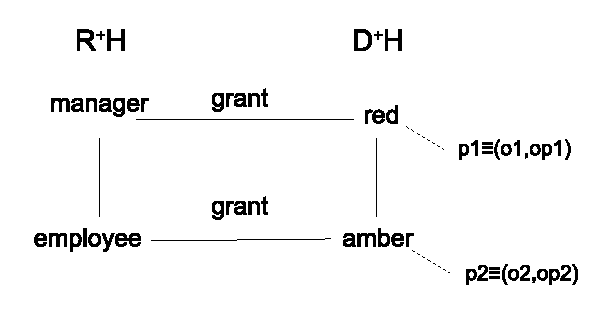
\includegraphics[width=.7\textwidth]{ABAC16/two-sorted-rbac-example}
 	\caption{An example of Two-sorted-RBAC}
 	\label{fig:two-sorted-rbac-example}
 \end{figure} 

 

The benefits of \twoSortedRBAC{} can also be realized through LaBAC. For example, user to $\uLabel{}$ value assignments, object to \oLabel{} value assignments and authorization policies are analogous to $\properRoleHierarchy$, $\demarcationHierarchy$ and grant relation in \twoSortedRBAC{} and  can also be carried out independently. On the other hand, many-to-many administrative mutation can also be achieved. For example, the LaBAC policy, $\Policy_{op1}\equiv \{(manager, (red,op1))\}$ in Figure \ref{fig:two-sorted-rbac-to-labac-example},  enables every   $manager$ to perform operation $op1$ on every object labeled with  $(red,op1)$. 

 \begin{figure}
 	\centering
 	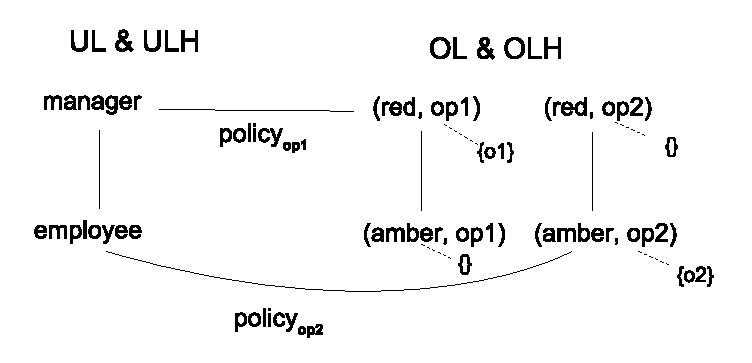
\includegraphics[width=.7\textwidth]{ABAC16/two-sorted-rbac-to-labac-example}
 	\caption{An example of Two-sorted-RBAC configured in LaBAC}
 	\label{fig:two-sorted-rbac-to-labac-example}
 \end{figure}
 


 \begin{table}
	\centering
	\caption{ \twoSortedRBAC{} in \hlabac} %\vspace*{3pt}
	\label{tab:two-sorted-rbac-in-labac-table}
	\begin{tabular}{|l|}						
		\hline					
		\multicolumn{1}{|c|}{\underline{\textit{I. \twoSortedRBAC{} components }}}\\	\\			 
		 -  $S, OBS, OPS$, $\roles, \RH$, $\demarcation, \DeH$,   (users, objects,   operations, proper roles, \\ \hfill role hierarchy, demarcation  and demarcation hierarchy respectively). \\
		 -  $PRMS = {(OBS \times OPS)}$, the set of permissions  \\		 
		 -  $\SR \subseteq S \times \roles$  \\
		 -  $\PD \subseteq PRMS \times \demarcation$ \\	 
		 - $G \subseteq \roles \times \demarcation$\\
		\\ \multicolumn{1}{|c|}{\underline{\textit{II. Construction in \hlabac{}}}} \\ \\
		 	-  $U = S, O = OBS, A = OPS $ \\ 
		 	- $UL=\roles, ULH=\RH$\\		  
		 	- $ OL = \demarcation \times OPS$\\
		 	- $OLH= \{ ((d_i, op_i), (d_j, op_j)) | d_i  \succeq d_j \land op_i = op_j\}$\\
		 	-  $\uLabel(u) = \{ r | (s,r) \in \SR \}$ \\		 	
		 	-  $ \oLabel(o) = \{ (d,op) | ((o,op),d) \in PD \}$\\		 	 	
		 	-  $\policy_{op_i} = \{ (r_i, (d_j,op_j) ) |  (r_i,d_i) \in G \land$ $((o,op_i),d_i)  \in \PD \} $ \\
		 \hline	
	\end{tabular}	

	
\end{table}

 
 In fact, LaBAC is similar to \twoSortedRBAC{} in spirit. While \twoSortedRBAC{} is more role oriented, LaBAC is attribute oriented. In the following of this section, we show equivalence of LaBAC and \twoSortedRBAC{} with respect to their theoretical  expressive power. In order to establish the equivalence, we show that any instance of \twoSortedRBAC{} can be expressed in LaBAC and vice-versa.

 
 
Figure  \ref{fig:two-sorted-rbac-to-labac-example} is an example showing configuration of a \twoSortedRBAC{} instance (given in Figure \ref{fig:two-sorted-rbac-example}) in LaBAC. In Figure  \ref{fig:two-sorted-rbac-to-labac-example}, user-label values and its hierarchy directly corresponds to roles and role hierarchy in Figure \ref{fig:two-sorted-rbac-example}. On the other hand, object-label values correspond to Cartesian product of $\demarcation$ and $OPS$.   An object-label value $(d_i, op)$ dominates another object-label value $(d_j, op)$, if demarcation $d_i$ dominates demarcation $d_j$. For example, for demarcations \{$red$, $amber$\} and operations $\{op1,op2\}$ (of Figure \ref{fig:two-sorted-rbac-example}), four object-label values have been defined where $(red,op1)$ dominates $(amber,op1)$ because $red$ dominates $amber$.  For an object-label value $(d,op)$, we assign $(d,op)$ to the object $o$ to if $(o,op)$ is a permission in demarcation $d$. For example, object $o1$ is assigned the value $(red,op1)$ because $(o1,op1)$ is  a permission in demarcation $red$.  On the other hand, user-label values assigned to a user corresponds to his assigned proper roles. Finally, having assigned object-label and user-label values, for each grant relation $(r,d) \in G$,  we specify authorization policy $Policy_{op} \equiv \{(r,(d,op))\}$ so that object labeled with $(d,op)$ are accessed by users with role $r$ for operation $op$. For example, for the grant relation $(manager,red)$ in Figure \ref{fig:two-sorted-rbac-example}, we create a policy $Policy_{op1} \equiv \{(manager, (red,op1))\}$. We do not create  policy $Policy_{op2} \equiv \{(manager, (red,op2))\}$ because there is no permission defined with operation $op2$ in demarcation $red$. Table \ref{tab:two-sorted-rbac-in-labac-table} formally  shows this configuration.
 

 
 %  \begin{figure}[!htbp]
 	\centering
 	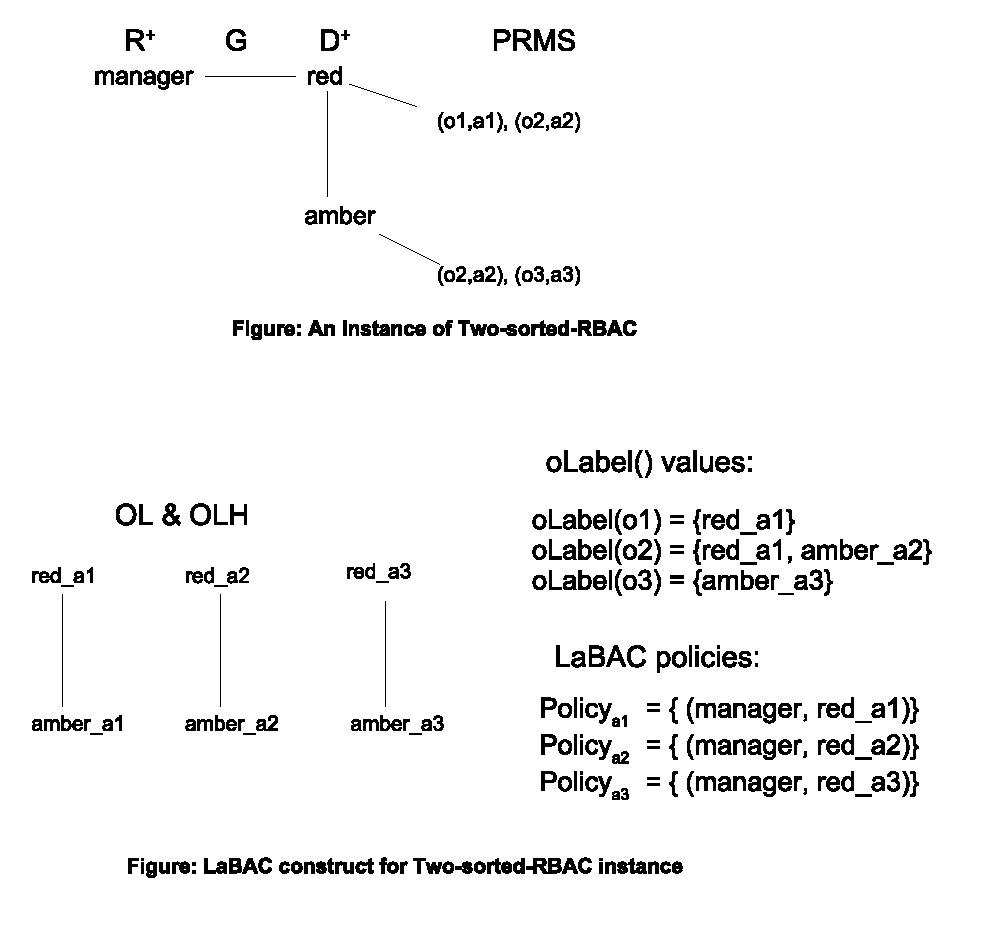
\includegraphics[width=.6\textwidth]{two-sorted-labac-example-diagram}
 	\caption{A $RBAC_1$ instance of role and perms.}
 	\label{fig:two-sorted-labac-example-diagram}
 \end{figure}
 
 \begin{table}
	\centering
	\caption{ \hlabac{} in \twoSortedRBAC{} } %\vspace*{3pt}
	\label{tab:labac-in-two-sorted-rbac-table}
	\begin{tabular}{|l|}						
		\hline					
			\multicolumn{1}{|c|}{\underline{\textit{I. \hlabac{} components}}} \\
			-  $U, O,  A$ (set of users, objects and actions resp.) \\ 
%			- $UL, OL, ULH,  OLH$ (uLabel and oLabel values, \\ \hfill uLabel and oLabel value hierarchy  resp.) \\		  
%			-  $\uLabel()$, user to user-label value assignment relation \\		 	
%			-  $\oLabel()$, object to object-label value assignment relation \\
%			-  $\policy_{a}$, LaBAC authorization policies for $a \in A$\\\\
			- $UL, OL, ULH,  OLH$ (uLabel values, oLabel values, \\ \hfill uLabel and oLabel value hierarchy  resp.) \\		  
			-  $\uLabel: U \to 2^{UL}$, $\oLabel: O \to 2^{OL}$ \\
			-  $\Policy_{a}$, authorization policy for action $a \in A$\\
		
		\\ \multicolumn{1}{|c|}{\underline{\textit{II. Construction in \twoSortedRBAC}}}\\	
		- $S=U, OBS=O, OPS=A$\\			 
		 - $\properRole = UL$, $\properRoleHierarchy = ULH$ \\ 
 		 - $\demarcation = OL$, $\demarcationHierarchy = \{\}$ \\ 
 		 - $\SR = \{ (u,r) | r \in uLabel(u)\}$\\
 		 - $\PD = \{ ((o_i, a_i), ol) | \exists (ul,ol) \in \policy_{a_i} \land$ \\ \hfill $ol' \in oLabel(o_i) \land ol \odominate ol'\}$ \\
 		 - $G = \{ (ul,ol) | (ul,ol) \in \policy_a  \}$\\
		\hline	
	\end{tabular}	

	
\end{table}

 
 
 
 Configuration of \hlabac{} in \twoSortedRBAC{} is given in Table \ref{tab:labac-in-two-sorted-rbac-table}. Segment I represents elements of LaBAC model and Segment II shows the configuration.  In the configuration, user-label values and its hierarchy are used as proper roles and proper role hierarchy. Object-label values are used as names for demarcations. For an object-label value $ol\in OL$, let $O_{ol}$ be the objects labeled with $ol$. For each policy $policy_{op} \equiv \{(ul, ol)\}$ in LaBAC, we create a grant relation $(ul,ol)$ in \twoSortedRBAC{}. Further, assign permission (o,op) in demarcation named $ol$ for $o \in O_{op}$. Note that \twoSortedRBAC{} does not distinguish between users and sessions as we do in LaBAC. For this reason, we omit LaBAC sessions while showing equivalence with \twoSortedRBAC{}.
 
 
 

  
  Here we use \hlabac{} to configure \twoSortedRBAC{} for convenience. In fact,  \clabac{} is the minimalistic model that is equivalent to \twoSortedRBAC{}. In Figure \ref{fig:expressiveness-spectrum}, we show summary of expressive power of different LaBAC models. The dashed box represents the minimalistic LaBAC model required to configure other models and solid box represents the LaBAC model that we use for our convenience. 

%We acknowledge the more formal  approach of \textit{state matching reduction} or simply \textit{reduction} \cite{tripli} for establishing equivalence between access control models. For simplicity and absence of state transition functions (administrative models) for some models discussed here, we adopt a simplified and conventional approach for the establishment of  equivalence.

The construction of Tables \ref{tab:two-sorted-rbac-in-labac-table} and \ref{tab:labac-in-two-sorted-rbac-table} and other constructions given in the rest of this paper can be cast in the formal approach of \cite{tripli}. So, these models are equivalent in the sense of state-matching reduction. 

   \begin{figure}
 	\centering
 	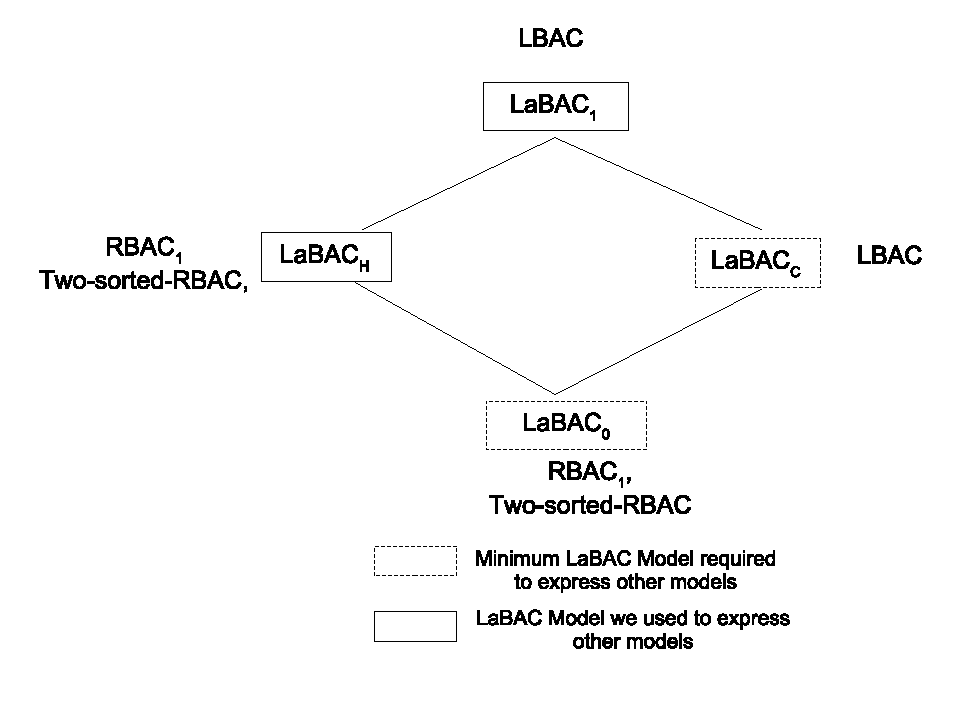
\includegraphics[width=.8\textwidth]{ABAC16/expressiveness-spectrum}
 	\caption{Expressiveness of LaBAC models}
 	\label{fig:expressiveness-spectrum}
 \end{figure}
 



%\section{LBAC and RBAC in  LaBAC}
\label{sec:configuration}
In this section, we configure LBAC \cite{lbac} and RBAC \cite{rbac}  using \labacOneOneOne{}. For each configuration, we additionally show the required number of label values and authorization policies. 

\newcommand{\latticeHead}{latticeTop} 
\newcommand{\securityClass}{SC}
\newcommand{\liberalStar}{\textit{liberal $\star$-property}}
\newcommand{\strictStar}{\textit{strict $\star$-property}}
%\subsection{LBAC in \labacOneOneOne} 




LBAC or Lattice Based Access Control is characterized by one directional information flow in a lattice of security classes. The security classes are partially ordered. One security class from these classes is assigned to each user which is known as clearance of the user. A user having a senior security class can also exercise his/her privileges using a junior  security class. For example, a top secret user can also exercise his privileges as secret user but he/she cannot use both secret and top secret clearance at the same time.  On the other hand, one security class (from the same classes of the security lattice) is assigned on objects commonly known as classification of the object. LBAC enforces one direction of information flow by two mandatory rules for reading and writing of these objects. One rule, known as \textit{simple-security property} (informally, read down rule), states that a subject (or user) can read an object if subject's clearance dominates object's classification. The other rule, known as \textit{liberal $\star$-property} (informally, write up rule),  states that a subject can write on an object if object's classification dominates subject's clearance. As a security class dominates itself it is possible to read and write  at the same level. A variation of \textit{liberal $\star$-property}, know as \textit{strict $\star$-property}, mandates that a subject can only write at his own level for the purpose of integrity requirements. A definition of LBAC is given in Segment I of Table \ref{tab:lbac-in-labac}.

\newcommand{\userLBAC}{U_{L}}
\newcommand{\objectLBAC}{O_{L}}
\newcommand{\sessionLBAC}{S_{L}}
\newcommand{\sessionUser}{sub\_creator}
\newcommand{\clearance}{clearance}
\newcommand{\classification}{classification}

\begin{table}
	\centering
	\caption{ LBAC in \labacOneOneOne{}} %\vspace*{3pt}
	\label{tab:lbac-in-labac}
	\begin{tabular}{|l|}						
		\hline					
		\multicolumn{1}{|c|}{\underline{\textit{I. LBAC components }}}\\	\\			 
		 - $\userLBAC, \objectLBAC$ and $\sessionLBAC$ (set of users, objects and sessions resp.) \\
		 -  \textit{SC}:  set of security classes in the lattice \\
		 -  \textit{SCH}: partial order on \textit{SC} (also denoted by $\succeq$ ) \\
		 - $\sessionUser: \sessionLBAC \to \userLBAC$, many-to-one mapping  from $\sessionLBAC$ to $\userLBAC$\\
		 - $\clearance: (\userLBAC \cup \sessionLBAC) \to SC$,  and  $clearance(s) \preceq \clearance(\sessionUser(s))$\\
		 - $\classification: \objectLBAC \to SC$\\		
	
		 - \textit{Simple-security property}: Subject s can read object o \\ \hfill only if \textit{clearance(s) $\succeq$ classification(o)}\\
		 - \textit{Liberal $\star$-property}: Subject s can write object o\\ \hfill only if  \textit{clearance(s) $\preceq$ classification(o)}\\
		  - \textit{Strict $\star$-property}: Subject s can write object o\\ \hfill only if  \textit{clearance(s) = classification(o)}\\
%		  - $createSession(u:\userLBAC,s:\sessionLBAC, sc:SC)$ \\ \hfill condition:$ s \not \in \sessionLBAC \land \clearance(u) \succeq sc$ \\ \hfill \hfil update: $\sessionLBAC' = \sessionLBAC \cup s$\\
		  
		  	\\	  \multicolumn{1}{|c|}{\underline{\textit{II. Construction in \labacOneOneOne{} }}} \\ \\
		  
		\\	  \multicolumn{1}{|l|}{{\textit{II(a). Construction of basic sets and relations }}} \\
		 - $U = \userLBAC, O = \objectLBAC, S = \sessionLBAC, A=\{read, write\}$\\
		 
		 - $\creator(s) = \sessionUser(s)$, for $s \in S$\\
		 -  $UL = SC,  ULH = SCH$ \\
		 - $OL = \{sc | sc \in SC \} \cup \{sc' | sc \in SC \}$\\
		 - $OLH=\{ (sc_i, sc_j) | sc_i \succeq sc_j \} \cup \{ (sc_i', sc_j') | sc_j' \succeq sc_i'\} $  [\liberalStar{}]\\
		 - $OLH=\{ (sc_i, sc_j) | sc_i \succeq sc_j \} $  [\strictStar{}]\\
		 -  $  \uLabel(u) =  clearance(u)$ \\
		 -  $  \oLabel(o) =  \{ sc, sc'\}$, where $sc=\classification(o)$	\\
		 - $ \Policy_{read} = \{ (sc_i, sc_i)| sc_i \in SC \}$ \\
		 - $ \Policy_{write} = \{ (sc_i, sc_i')| sc_i \in SC  \}$ \\
		% - Def. of  $\impliedPolicy_{op_i}$,  $\sessionLabels(s)$ for session $s \in S$ \\ \hfill and $\request(s, a, o)$  are unchanged from Table \ref{tab:labac-definition}	\\	
		 %- Session Constraints: $|\sessionLabels(s)  \cap SC| = 1$
		 
		 \\ \multicolumn{1}{|l|}{{\textit{II(b). Condition on session functions}}} \\ \\
		 - $f_{\createSession} (u, s, val) : |val|=1$\\
		 - $f_{\deleteSession}(u,s): true$\\
	     - $f_{\assignValues} (u, s, val): false$ [assuming tranquility]\\
	     - $f_{\removeValues} (u, s, val): false$ [assuming tranquility]\\
	     
	     \\ \multicolumn{1}{|c|}{\underline{\textit{III. LaBAC extension for object creation}}} \\
	     - $\createObject(s,o,\{val\})$: create a new object, and    assign value $\{val\}$\\
		    \hspace{5em} condition: $s \in S \land o \not \in O \land \exists ul  \in \sessionLabels(s)  $  $ \land val \succeq ul]$ \\
		      \hspace{5em} update: $O' = O \cup \{o\}, \oLabel(o) = \{val\}$ \\
%		 - $\updateObject(s,o,\{val\})$: update $\oLabel$ value \\ \hfill of existing object\\
%		 \hfil condition: $s \in S \land o \in O \land \exists ol, \exists ul [\sessionLabels(s)=ul \land$ \\ \hfill $  \oLabel(o) = ol \land ul \udominate ol \land ul \udominate val ]$ \\
%		   \quad  update: $ \oLabel(o) = \{val\}$ 
	 \hline	
	\end{tabular}	
\end{table}



 

We present the configuration of LBAC in  \labacOneOneOne{}. Minimalistically, we need \consLabac{}  to configure some constraints of LBAC, for example, at most one security class can be activated by a subject (i.e. session in case of \eapABAC{} ) at a time. We use \labacOneOneOne{} for convenience.  

 The configuration of LBAC in \labacOneOneOne{} is given in Segment II of Table \ref{tab:lbac-in-labac}.  The security classes and its hierarchy are directly used as user label values and its hierarchy. For object-label values and its hierarchy we consider both the original lattice and the inverted lattice. The clearance of a user in LBAC  is assigned as $\uLabel$ values of the user in \eapABAC{} . On the other hand, if an object has a classification of $sc \in SC$ in LBAC,  we assign the object $\oLabel$ values of \{\textit{sc,sc'}\}, where $sc'$ correspond to $sc$ in the inverted lattice.  The \textit{simple-security} property is configured as a \eapABAC{}  policy  $\Policy_{read} \equiv \{(sc_i, sc_i)\}$ so that users having user-label value $sc_i$ can read objects having object-label value $sc_i$ or its junior.  Similarly, the $\star$-\textit{property} is configured with $\Policy_{write} \equiv \{(sc_i, sc_i')\}$ where $sc_i$ is the user-label value from the original lattice and $sc_i'$ is the object-label value from the inverted lattice and  $sc_i$  correspond to $sc_i'$. For the \liberalStar, we consider the hierarchy of the inverted lattice where as we do not consider them for the \strictStar.  An example of LBAC configured in \labacOneOneOne{} is given in Figure \ref{fig:lbac-labac-example}.

 \begin{figure}
 	\centering
 	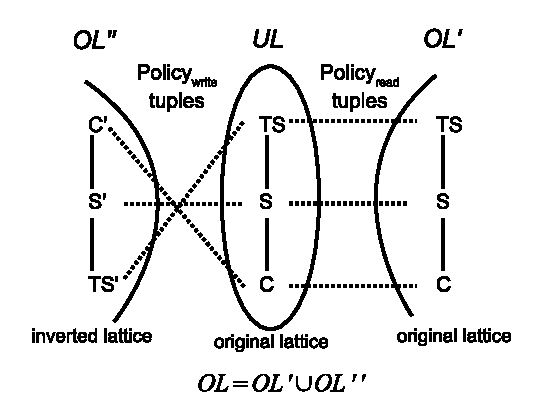
\includegraphics[width=.4\textwidth]{ABAC16/lbac-labac-example}
 	\caption{LBAC example configured in LaBAC}
 	\label{fig:lbac-labac-example}
 \end{figure}
\begin{table} 
	\centering
 \caption{Quantifying \eapABAC{} for simulating LBAC}
 \label{tab:lbac-labac-quantification}
	\begin{tabular}{|l|}
		\hline	                                                                                                           	

		$|UL| = |SC|$ and $|OL| =  2 |SC|  $\\
		$|\Policy| = 2$  $(|\Policy_{read}| $ and $|\Policy_{write}|)$\\
		%|\policy_{read}| =  1$\\
		%|\policy_{write}| =  1$\\
		\hline
		\end{tabular}  

\end{table}

Segment II(b) of Table \ref{tab:lbac-in-labac} specifies conditions for the session management functions in \eapABAC{} . In  $\createSession()$ we specify additional condition so that at most one user-label value can be activated in one session. We assume, once created clearance of subjects and classification of objects cannot be changed. This property in known \textit{tranquility} in the literature \cite{lbac}
  
Segment III is an extension of \labacOneOneOne{} for the purpose of creating objects in \eapABAC{} . Since functional specification of \labacOneOneOne{} does not include functions for creating or managing objects,  here we define a function $\createObject()$ for this purpose. We follow the \liberalStar{} as the precondition for creation of objects. 

%and $\updateObject()$ to capture creation of new objects and modification of object classification values in LBAC. The prerequisite conditions and necessary updates for execution of these functions are also presented here. 


Finally, Table \ref{tab:lbac-labac-quantification} shows required number of authorization policies, $UL$ and $OL$ values  for configuring LBAC.

%to configure LBAC in \labacOneOneOne{}.

%we quantify required number of required \labacOneOneOne{} policies for configuring LBAC which is shown in Table \ref{tab:lbac-labac-quantification}. As we can see, we need as many read and write policies as the number of security classes in the lattice.



 

 % \begin{figure*}
 	\centering
 	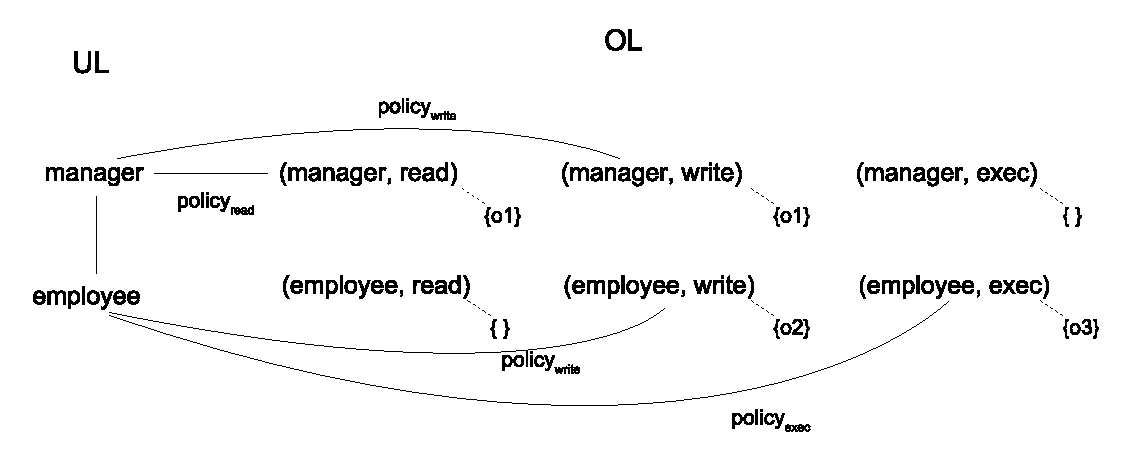
\includegraphics[width=.8\textwidth]{ABAC16/rbac-labac-configuration-explained}
 	\caption{An instance of RBAC (from Figure \ref{fig:rbac-labac-example}) configured in LaBAC.}
 	\label{fig:rbac-labac-configuration-explained}
 \end{figure*}
 \newcommand{\associatedObj}{associated\_obj}

 \begin{figure}
 	\centering
 	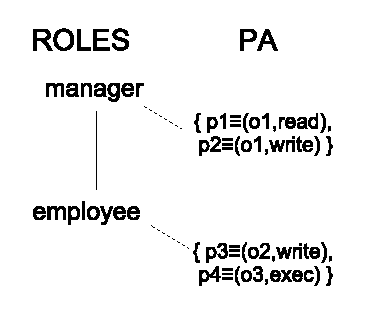
\includegraphics[width=.3\textwidth]{ABAC16/rbac-labac-example}
 	\caption{An example of roles and permission-role assignments in RBAC.}
 	\label{fig:rbac-labac-example}
 \end{figure}
 \begin{figure*}
 	\centering
 	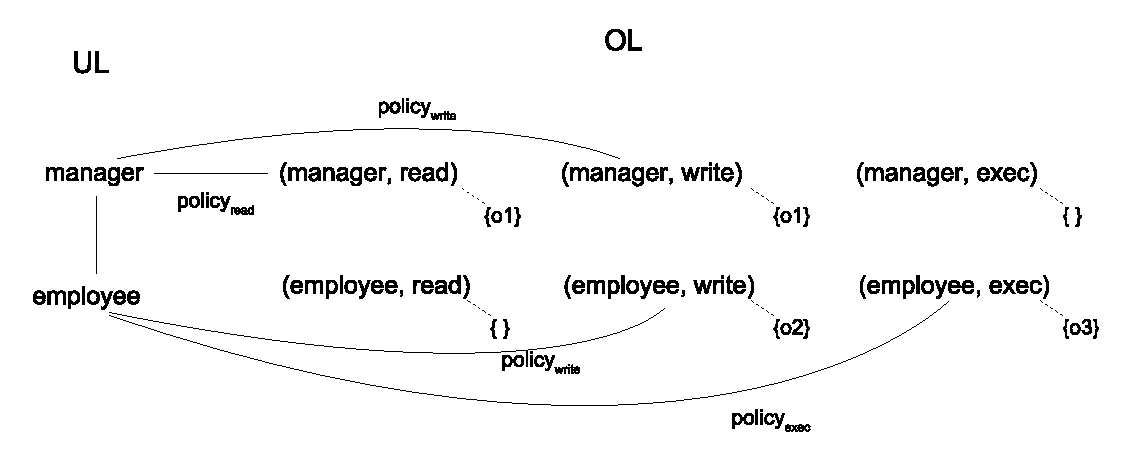
\includegraphics[width=.8\textwidth]{ABAC16/rbac-labac-configuration-explained}
 	\caption{An instance of RBAC (from Figure \ref{fig:rbac-labac-example}) configured in LaBAC.}
 	\label{fig:rbac-labac-configuration-explained}
 \end{figure*}


 
%\begin{table}[]
\centering
\caption{Authorization policies in \hlabac{}  illustrating roles  in Figure \ref{fig:rbac-labac-example}}
\label{tab:rbac-labac-example-table}
\begin{tabular}{|l|l|l|l|}
	\hline
UL  & OL                                                                   & oLabel(o)                                                                          & Policy                                                                                                                                               \\
\hline
mng & \begin{tabular}[c]{@{}l@{}}\{mng\_read,\\ mng\_write\}\end{tabular}  & \begin{tabular}[c]{@{}l@{}}oLabel(o1)=\\ \{mng\_read, \\ mng\_write\}\end{tabular} & \begin{tabular}[c]{@{}l@{}} $p_{read} \equiv$ \\$\{(mng, mng\_read) \}$,\\ $p_{write} \equiv$ \\ $\{(mng, mng\_write)$,\}\end{tabular} \\ 
\hline
emp & \begin{tabular}[c]{@{}l@{}}\{emp\_write, \\ emp\_exec\}\end{tabular} & \begin{tabular}[c]{@{}l@{}}oLabel(o2)=\\ \{emp\_write, \\ emp\_exec\}\end{tabular} & \begin{tabular}[c]{@{}l@{}}$p_{read} \equiv$ \\ $\{(emp, emp\_write)\}$,\\ $p_{exec} \equiv $ \\ $\{(emp,  emp\_exec)\}$\end{tabular}       \\
\hline                                               
\end{tabular}
\end{table}



\newcommand{\sessionRoles}{session\_roles}
\begin{table}
	\centering
	\caption{ $RBAC_1$ in \hlabac} %\vspace*{3pt}
	\label{tab:rbac-in-labac-table}
	\begin{tabular}{|l|}						
		\hline					
		\multicolumn{1}{|c|}{\underline{\textit{I. $RBAC_1$ components }}}\\				 
		 -  \textit{USERS, OBS, OPS, SESSIONS, ROLES} and \textit{RH} \\ \hfill (users,  objects, operations, sessions, roles \\ \hfill and role hierarchy resp.) \\
		 -  $\textit{PRMS} = {(\textit{OBS} \times \textit{OPS})}$, the set of permissions  \\		 
		 -  $\textit{UA} \subseteq \textit{USERS} \times \textit{ROLES}$.  \\
		 - $\textit{PA} \subseteq \textit{PRMS} \times \textit{ROLES}$. \\	
		 - $session\_user: \textit{SESSIONS} \to USERS$ \\
		 %- $\sessionRoles: \textit{SESSIONS} \to 2^{\textit{ROLES}}$ ; $\sessionRoles(s) \subseteq$ \\ \hfill  $  \{r | (\exists r' \succeq r)[session\_user(s),r') \in \textit{UA}]\}$\\
		  - $\sessionRoles: \textit{SESSIONS} \to 2^{\textit{ROLES}}$ and \\ \hfill $\sessionRoles(s) \subseteq  \{r | (\exists r' \succeq r)[session\_user(s),r') \in \textit{UA}]\}$\\
		\\\multicolumn{1}{|c|}{\underline{\textit{II. Construction in \hlabac}}} \\
		 	-  $U = \textit{USERS}, O = \textit{OBS}, A = \textit{OPS}, S=\textit{SESSIONS} $ \\ 
		 	- \textit{UL=ROLES, ULH=RH}\\		  
		 	- $ OL = \textit{ROLES} \times \textit{OPS}$, $\textit{OLH}= \{ \}$\\
		 	-  $\uLabel(u) = \{ r | (u,r) \in UA \}$ \\
		 	
		 	-  $ \oLabel(o) = \{ (r,op) | ((o,op),r) \in PA \}$\\
		 	- $\creator(s) = session\_user(s)$, for $s \in S$	\\
		 	- $\sessionLabels(s) = \sessionRoles(s)$, for $s \in S$\\
		 	-  $\policy_{op_i} = \{ (r, (r',op_i) ) |  ((o,op_i),r')  \in PA \land r' = r  \} $ \\
		 	%- $\impliedPolicy_{op_i}$ and $\request()$ functions  are \\ \hfill unchanged from Table \ref{tab:labac-definition}	\\	
		 	
%		 	 \\ \multicolumn{1}{|c|}{\underline{\textit{III. Condition on session functions}}} \\
%		 	 - $\createSession(u,s,values)$: \\ \hfil $u \in U \land s \not \in S \land values \subseteq \uLabel(u)$\\
%		 	 - $\deleteSession(u,s)$: \\ \hfil $u \in U \land s \in S \land \creator(s)=u$\\
%		 	 - $\assignValues(u,s,values)$: \\ \hfil $u \in U \land s \in S \land \creator(s)=u \land values \subseteq \uLabel(u)  $ \\ 
%		 	 - $\removeValues(u,s,value)$: \\ \hfil $u \in U \land s \in S \land \creator(s)=u \land value \subseteq \uLabel(u)$ \\
		 	
		 \hline	
	\end{tabular}	

	
\end{table}

 
%\subsection{RBAC in \hlabac} 
A definition of hierarchical RBAC ($RBAC_1$) is shown in Segment I of Table \ref{tab:rbac-in-labac-table}. In RBAC, permissions are assigned to roles and users receive permissions through their enrollment to roles. Roles are partially ordered. If a role, $r_i$ is senior to role, $r_j$ (otherwise told $r_i$ dominates $r_j$), $r_i$ inherits permissions from $r_j$ and $r_j$ inherits users from $r_i$. Thus role hierarchy serves dual purpose of inheriting users and permissions. Figure \ref{fig:rbac-labac-example} presents an example showing roles, role hierarchy and permission-role assignments in $RBAC_1$. 

In Segment II of Table \ref{tab:rbac-in-labac-table}, we show  construction of $RBAC_1$ in \hlabac. Minimalistically, we need \clabac{}, but we use \hlabac{} for convenience. 



Figure  \ref{fig:rbac-labac-configuration-explained} shows an instance of RBAC (given in Figure \ref{fig:rbac-labac-example}) configured in \eapABAC{}. In the figure, user-label values and its hierarchy directly correspond to roles and role hierarchy of Figure \ref{fig:rbac-labac-example}. On the other hand, object-label values correspond to Cartesian Product of $ROLES$ and $OPS$.   For example, for roles \{$manager, employee$\} and operations $\{read, write, exec\}$ of Figure \ref{fig:rbac-labac-example}, six different object-label values have been defined.  For an object-label value $(r,op)$, we assign it to the object $o$  if $(o,op)$ is a permission assigned to role $r$. For example, object $o1$ is assigned to label $(manager,read)$ because $(o1,read)$ is  a permission of role $manager$ (see Figure \ref{fig:rbac-labac-example}). Having assigned object-label and user-label values, for each $r \in ROLES$,  we specify authorization policy $\Policy_{op} \equiv \{(r,(r,op))\}$ so that object labeled with $(r,op)$ are accessed by users labeled with role $r$ for operation $op$. For example, for role, $manager$ in Figure \ref{fig:rbac-labac-example}, we create $\policy_{read} \equiv \{(manager, (manager,read))\}$ and $\policy_{write} \equiv \{(manager, (manager,write))\}$. We do not create  policy $\policy_{exec} \equiv \{(manager, (manager, exec))\}$ because there is no permission defined with operation $exec$ in role $manager$. Table \ref{tab:rbac-in-labac-table} formally shows the configuration of $RBAC_1$ in \eapABAC{}. 




\begin{table} 
	\centering
 \caption{Quantifying \eapABAC{} for simulating RBAC}
 \label{tab:rbac-labac-quantification}
 
 	\begin{tabular}{|l|}
 		\hline	                                                                                                           	
 		
 	$|UL| = |ROLES|$\\ 
 	$|OL| = |ROLES| \times |OPS|$\\
 	$|\Policy| = |OPS|$\\
 		\hline
 	\end{tabular}  
\end{table}
 
 

 
 Finally, Table \ref{tab:rbac-labac-quantification} presents number of user-label values, object-label values and authorization policies required to configure $RBAC_1$.  
 


 





%\subsection{DAC in \clabac}

 
% Please add the following required packages to your document preamble:
% \usepackage{booktabs}
\begin{table*}
	\centering
	\caption{ DAC in \labacOneOneOne{} for finite users and objects} %\vspace*{3pt}
	\label{tab:dac-definition}
	\begin{tabular}{|l|}						
		\hline					
	 
		\multicolumn{1}{|c|}{\underline{\textit{I. Construction}}} \\
		- let $OID$ be finite set of object ids. \\
		-  $U, A$, be finite set of users, and actions\\
		- $O$, set of existing objects. \\
		-   $OL=OID$, $UL=\{ id(u) | u \in U \}$, for \\ \hfill $id(u)$ as the unique id of a user. \\
		- $\policy$, set of existing policies.\\
		\multicolumn{1}{|c|}{\underline{\textit{II. Administrative Actions Required for DAC}}} \\
			- let $\canAddPolicy \subseteq U \times 2^{UL} \times A \times 2^{OL}$, \\  \hfill be an administrative relation.  $(au, X, a, Z) \in \canAddPolicy$ \\  \hfill implies that  administrative user, $au$  can add/remove \\ \hfill  policy,  $policy_a \equiv (x:X,z:Z)$\\
		\multicolumn{1}{|c|}{\underline{\textit{III. create new object}}} \\
			- $create\_object(u:U, oid:OID)$ \{ \\
			\quad $o = create\_new(oid)$ \\
			\quad	$oLabel(o) = \{oid\}$\\
			\quad	$\policy = \policy \cup \{ ( id(u), read, oid), ( id(u), write, oid) )\}$ \\
			\quad   $\canAddPolicy = \canAddPolicy \cup \{(u, UL, A, \{oid \}) \}$ \\		
			\quad \} \\
			\hline
	\end{tabular}	
\end{table*}



\input{labac-in-PM-mini.tex}
%\section{Comparative Analysis of the ABAC Models}
	
	
	\subsection{Abstract Policy \& Policy Space}
	\newcommand{\uSubset}{U_S}
\newcommand{\oSubset}{O_S}
\newcommand{\UAExpr}{UAExpr}
\newcommand{\OAExpr}{OAExpr}
\newcommand{\uSelector}{USERs}
\newcommand{\oSelector}{OBJECTs}
\newcommand{\policySpace}{PolicySpace}

  \begin{table} 
\centering
\caption{One abstract policy represented by different \sABAC{} policies}
\label{table:sabac-def}
\begin{tabular}{@{}l@{}}
 \toprule	
	 $  E(role(u), \{manager, employee\}) \land E(type(o),\{new\} )$\\
	 $  E(role(u), \{manager\}) \land E(role(u), \{employee\}) \land E(type(o),\{new\} )$\\
	 $ \lnot E(role(u), \{\}) \land E(role(u), \{employee\}) \land E(type(o),\{new\} )$\\
 	 $ \lnot (\lnot (E(role(u), \{manager, employee\}))) \land E(type(o),\{new\} )$\\
 \bottomrule
\end{tabular}
\end{table}
 
 \textbf{Abstract Policy}
 We define abstract policy as a tuple of following forms - $(\uSubset, a, \oSubset)$ and $(\UAExpr, a, \OAExpr)$, where $\uSubset \subseteq U$ and $\oSubset \subseteq O$, $\uSelector(\UAExpr) \subseteq U$ and $\oSelector(\OAExpr) \subseteq O$, for function $\uSelector()$ and $\oSelector()$ which specifies set of users and objects for given user attribute expression and object attribute expression. Examples of abstract policy are $(\{ Alice, Bob\}, read, \{ o1, o2\} )$ or $( E(role(u), \{manager \}), read, E(\{ type(o), \{sensitive\} ) ) $
 
 We say two abstract policies $\rho_i \equiv (\UAExpr_i, a, \OAExpr_i)$ and   $\rho_j \equiv (\UAExpr_j, a, \OAExpr_j)$ are different ($\rho_i \neq \rho_j$) iff either or both of following conditions are true.
 \begin{enumerate}
 	\item $\uSelector(\UAExpr_i) \neq  \uSelector(\UAExpr_j) \lor U_i \neq U_j$  
 	\item $\oSelector(\OAExpr_i) \neq  \oSelector(\OAExpr_j) \lor O_i \neq O_j$
 \end{enumerate}

Informally, \policySpace{} of an model is the set of all distinct abstract policies of the model. For simplicity, here we are only interested about the size of the \policySpace{}.

	\begin{figure} 
		\centering
		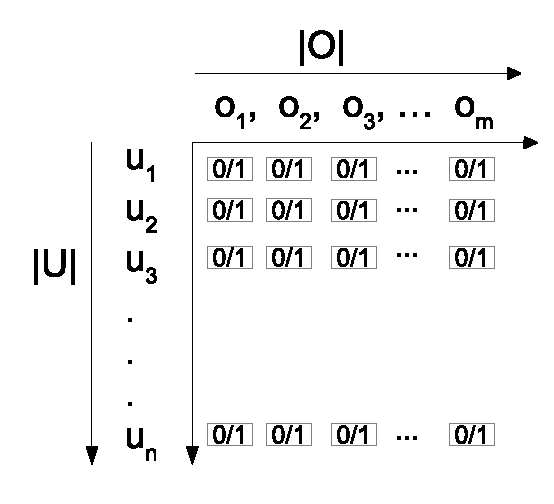
\includegraphics[width=.4\textwidth]{policyspace-hru}
		\caption{LaBAC with one object label and one user label}
		\label{fig:policyspace-hru}
	\end{figure}
 	\begin{figure} 
 		\centering
 		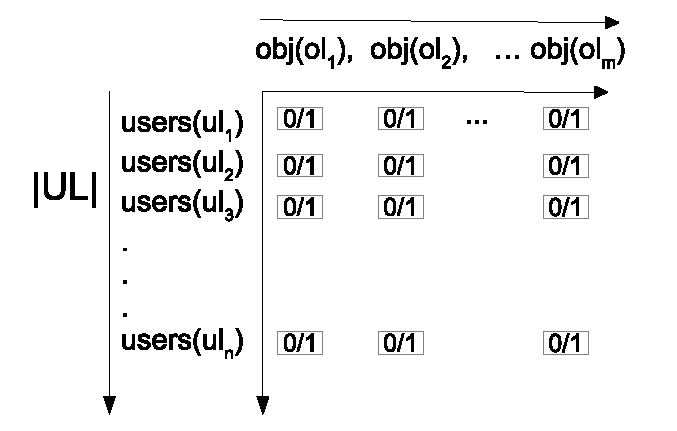
\includegraphics[width=.4\textwidth]{policyspace-labac1}
 		\caption{LaBAC with one object label and one user label}
 		\label{fig:policyspace-labac1}
 	\end{figure}
 	\begin{figure} 
 		\centering
 		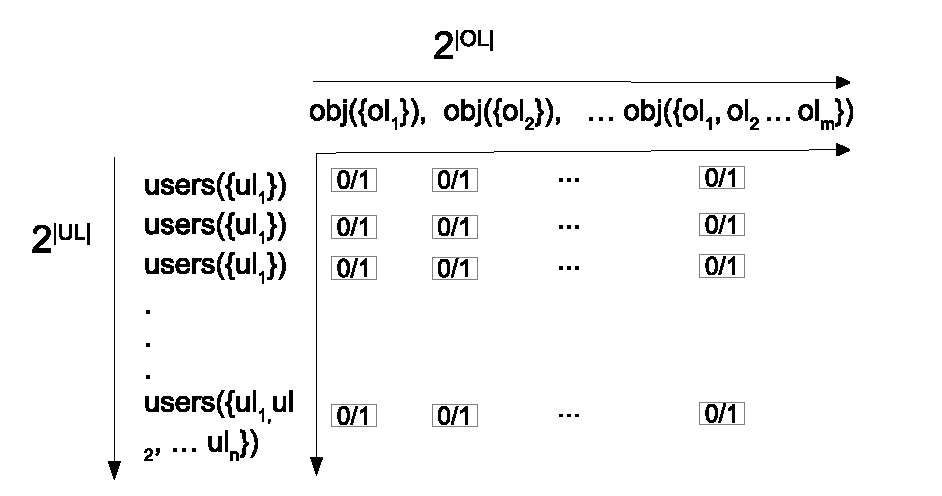
\includegraphics[width=.4\textwidth]{policyspace-labace}
 		\caption{LaBAC with one object label and one user label}
 		\label{fig:policyspace-labace}
 	\end{figure}
% Please add the following required packages to your document preamble:
 % \usepackage{booktabs}
 \begin{table}
 	\centering
 	\caption{Comparison of \policySpace{}}
 	\label{tab:policyspace-comparison}
 	\begin{tabular}{|l|l|}
 		 \hline
 		\textit{HRU \cite{hru}} & $ 2 ^{|U| \times |O|}$ \\
 		\textit{\labacOneOneOne{} } & $ 2 ^{|UL| \times |OL|}$ \\
 		\textit{\elabac} & $ 2 ^{2^{|UL|} \times 2^{|OL|}}$ \\
 		\textit{$\abacAlpha{} \cite{abacAlpha}$} & $2 ^{32}$ \\
 		\textit{\hgabac{}* \cite{hgabac}} & $ 2 ^{2^{|ua_1|} \times 2^{|oa_1|}}$ \\
\hline
 	\end{tabular}
 \end{table} 

 
						
 
%\section{Extensions of LaBAC Model}


\subsection{Extended Policy Model (\elabac)}
% Please add the following required packages to your document preamble:
% \usepackage{booktabs}
\begin{table}
	\centering
	\caption{ \elabac{} Model} %\vspace*{3pt}
	\label{tab:labac-definition}
	\begin{tabular}{|l|}						
		\hline					
		\multicolumn{1}{|c|}{\underline{\textit{I'. New/updated components of the extended model } } }\\	
		- $NUL$ and $NOL$ (set of negated user-labels and \\ \hfill negated object-labels).  $NUL = \{ \lnot ul | \exists ul \in UL\}$ and \\ \hfill  $NOL = \{ \lnot  ol | \exists ol \in OL \}$ \\
		%- $EUL$ and $EOL$ (extended set of user-labels and object-labels). \\ \hfill $EUL = UL \cup NUL$ and  $EOL = OL \cup NOL$ \\
		%- $uLabel$ and $oLabel$ are label functions on users and objects respectively. \\ \hfil Formally, $\uLabel(u:U) \to 2^{\UL}$ and $\oLabel(o:O) \to 2^{\OL}$ \\
		-  $\policy \subseteq 2^{UL \cup NUL} \times A \times 2^{OL\cup NOL}$. \\
		- An individual policy,  $p \in \policy$  \\ \hfil is enumeration of tuples of the form \\ \hfill  $( UL_s \subseteq  UL \cup NUL, a \in \A, OL_s \subseteq OL \cup NOL)$. \\
		%- $\sessionLabels(s:S) \to 2^{UL}$, mapping function from a session to the set of user-labels.  \\ \hfil Formally, 
		%$\sessionLabels(s) \subseteq \{ul' | ul \in uLabel(user(s)) \land ul  \udominate ul'  \}$.		\\ \\
		
	 		  
		
		\multicolumn{1}{|c|}{\underline{\textit{IV. Derived components}}} \\
		- $\impliedPolicy = \{ (UL_t, a, OL_t) | ( \exists (UL_s, a, OL_s) \in \policy) \land$  \\ \hfill $UL_t=\{ ul_j | ( ul_i \in UL_s \cap UL \land ul_j \udominate ul_i) \lor ul_j \in UL_s \cap NUL \} \land$ \\ \hfill $  OL_t=\{ ol_j | (ol_i \in OL_s \cap OL \land ol_i \udominate ol_j\}) \lor ol_i \in OL_s \cap NOL \}$		\\		
	 
		\multicolumn{1}{|c|}{\underline{\textit{V. Authorization functions}}} \\
		- \request(s:S,\amem:A,\objmem:O) =	\\ \hfill  $\exists (UL_s, a, OL_s) \in \policy \cup \impliedPolicy ] \land $   \\
		 \hfill   $\exists ul_i \in UL_s \cap UL \implies  ul_i \in \uLabel(u) \land$ \\
		 \hfill $\exists  ul_i \in UL_s \cap NUL \implies  ul_i \notin \uLabel(u)$ \\
		 \hfill   $\exists ol_i \in OL_s \cap OL \implies  ol_i \in \oLabel(o) \land$ \\
		 \hfill $\exists  ol_i \in OL_s \cap NOL \implies  ol_i \notin \oLabel(o)$ \\

		\\ \hline	
	\end{tabular}
	
\end{table}

%mod



 	\begin{figure}
 		\centering
 		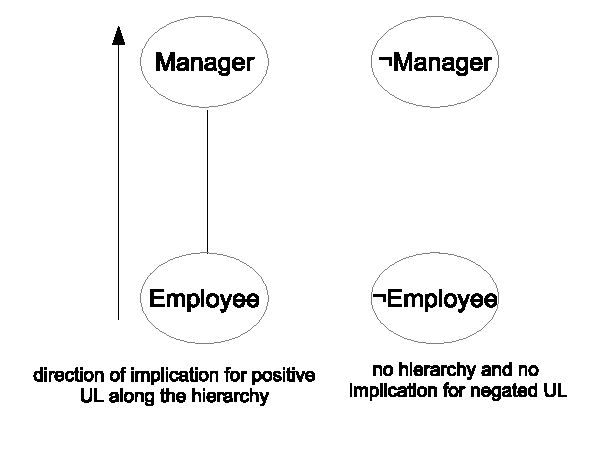
\includegraphics[width=.4\textwidth]{ul-implication}
 		\caption{Implication on UL}
 		\label{fig:ul-implication}
 	\end{figure}

 	\begin{figure} 
 		\centering
 		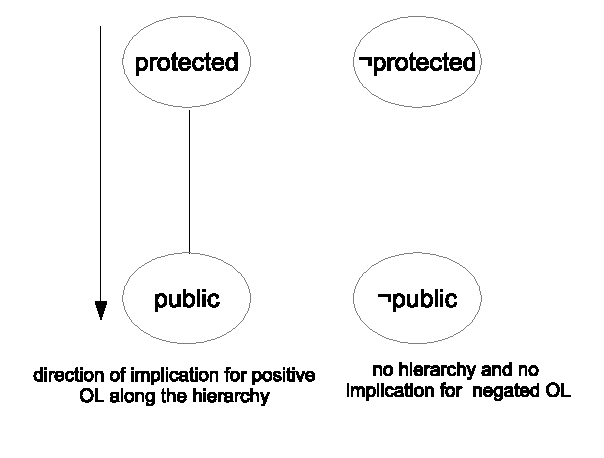
\includegraphics[width=.4\textwidth]{ol-implication}
 		\caption{OL Implication}
 		\label{fig:ol-implication}
 	\end{figure}

\subsection{Multi-label Extensions}
\newcommand{\OLOne}{OL_1}
\newcommand{\OLTwo}{OL_2}
\newcommand{\ULOne}{UL_1}
\newcommand{\ULTwo}{UL_2}
	\begin{figure*} 
		\centering
		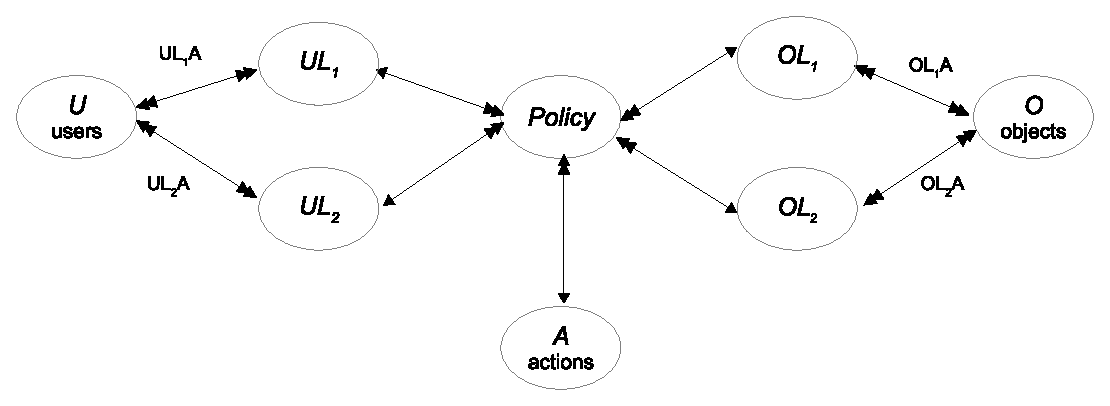
\includegraphics[width=.9\textwidth]{labac22}
		\caption{LaBAC with two object labels and two user labels}
		\label{fig:labac22}
	\end{figure*}

% Please add the following required packages to your document preamble:
% \usepackage{booktabs}
\begin{table}
	\centering
	\caption{ \labacZeroTwoTwo{} Model} %\vspace*{3pt}
	\label{tab:labac022-definition}
	\begin{tabular}{|l|}						
		\hline					
		\multicolumn{1}{|c|}{\underline{\textit{I. Component of the basic model }}}\\			
		- $U, O$, $A$ and $S$ (set of users, objects, actions and \\ \hfill sessions respectively).  \\
		- $\ULOne, \ULTwo, \OLOne, \OLTwo$ (set of $uLabel_1, uLabel_2,$ \\ \hfill $oLabel_1$ and $oLabel_2$ values respectively). \\
		- $\uLabelOne, \uLabelTwo, \oLabelOne, \oLabelTwo$ are label functions \\ \hfill on users and objects respectively. Formally, \\ \hfill  $\uLabelOne(u:U) \to 2^{\ULOne}$ and $\oLabelOne(o:O) \to 2^{\OL1}$ \\ \hfill  $\uLabelTwo(u:U) \to 2^{\ULTwo}$ and $\oLabelTwo(o:O) \to 2^{\OL2}$ \\  
		-  $\policy_a \subseteq \ULV_1 \times \ULV_2 \times \OLV_1 \times \OLV_2$ \\
		 %An individual policy,   $p \in \policy$  is \\ \hfil enumeration of tuples of the form $( ul_1 \in UL_1, ul_2 \in UL_2, a \in \A, ol_1 \in OL_1, ol_2 \in OL_2)$. \\
	 
		 - $\sessionLabels(s:S) \to 2^{UL_1 \times UL_2}$, mapping function from \\ \hfill a session   to the set  of $\uLabelOne{}$ and $\uLabelTwo{}$ values.    \\ \hfill formally	$\sessionLabels(s) \subseteq \{(ul_1', ul_2') | ul_1 \in \uLabelOne(user(s)) \land$ \\ \hfill $ul_1  \udominate ul_1' \land$   $ul_2 \in \uLabelTwo(user(s)) \land ul_2  \udominate ul_2' \}$.		\\ \\
		
		\multicolumn{1}{|c|}{\underline{\textit{V. Authorization functions}}} \\
		- \request(u:U,\amem:A,\objmem:O) =	 \\ \hfill
		$\exists ul_1 \in \uLabelOne(u) \land ul_2 \in \uLabelTwo(2) \land$ $ ol_1 \in \oLabelOne(o) \land$ \\ \hfill  $ ol_2 \in \oLabelTwo(o) \land  (ul_1, ul_2,ol_1, ol_2) \in \policy_a   $  

		\\ \hline	
	\end{tabular}
	
\end{table}

%mod



	\begin{figure} 
		\centering
		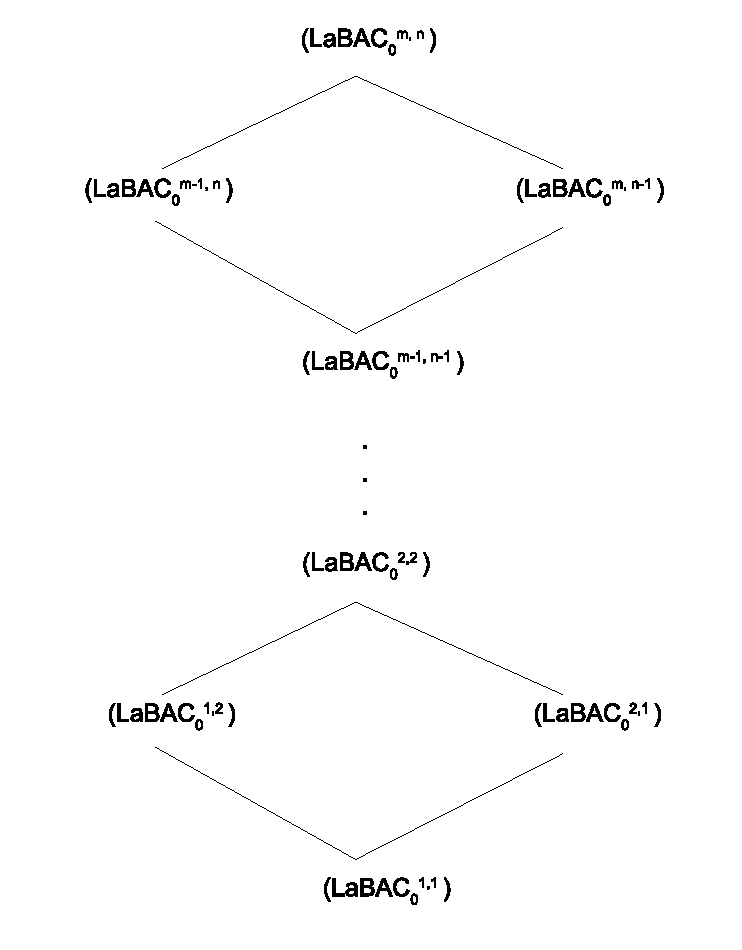
\includegraphics[width=.4\textwidth]{labacmn-family}
		\caption{LaBAC family of model extended with m object labels and n user labels.}
		\label{fig:labacmn-family}
	\end{figure}

\subsection{Expressive power of  \labacZeroOneOne vs \labacZeroMN}

% Please add the following required packages to your document preamble:
% \usepackage{booktabs}

\begin{table}
	\centering
	\caption{  \labacZeroTwoTwo{} in \labacZeroOneOne{}} %\vspace*{3pt}
	\label{tab:lbac-in-labac}
	\begin{tabular}{|l|}						
		\hline					
		\multicolumn{1}{|c|}{\underline{\textit{I. \labacZeroTwoTwo{} Components }}}\\	
		 - $U^{2,2}, O^{2,2}, A^{2,2}$	\\		 
	     - $UL_1, UL_2, OL_1, OL_2$\\
		 -  $\uLabelOne(), \uLabelTwo(), \oLabelOne(), \oLabelTwo()$ \\
		 -  $\policy^{2,2}_a \subseteq  UL_1 \times UL_2 \times OL_1 \times OL_2$\\	 
		\multicolumn{1}{|c|}{\underline{\textit{III. Construction}}} \\
		 - $U = U^{2,2}, O = O^{2,2}, A = A^{2,2}$\\
		 -  $UL = UL_1 \times UL_2$ \\
		 - $OL = OL_1 \times OL_2$\\		 
		 -  $  \uLabel(u) =  \uLabelOne(u) \cup \uLabelTwo(u)$ \\
		 -  $  \oLabel(o) =  \oLabelOne(o) \cup \oLabelTwo(o)$ \\ 
		 - $ \policy_{a} = \{ ( (UL_1 \times UL_2) \times (OL_1 \times OL_2))|$ \\ \hfill $(ul1, ul2, ol1, ol2) \in \policy_a \}$ \\
		 - Def. of  $\sessionLabels(s)$ for session $s \in S$  and \\ \hfill $\request(s, a, o)$   are unchanged 	\\	
	 
		\\ \hline	
	\end{tabular}	
\end{table}

%\section{Discussion on ABAC Policy}
%


\subsection { Implementation in OpenStack Swift}
\label{sec:implementation}

 \begin{figure} [t]
 	\centering
 	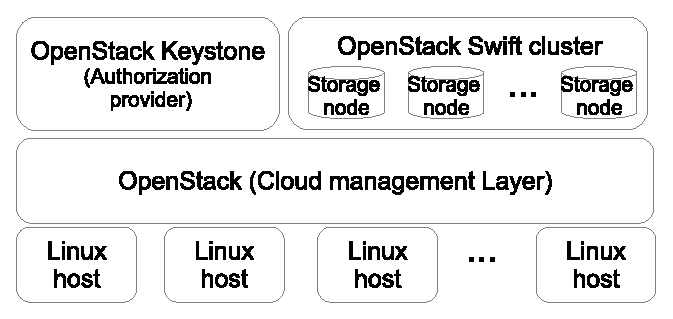
\includegraphics[width=.6\textwidth]{NSS16/reference-implementation-architecture}
 	\caption{Reference architecture of the implementation testbed}
 	\label{fig:reference-implementation-architecture}
 \end{figure}


 
 	\begin{figure} [t]
 		\centering
 		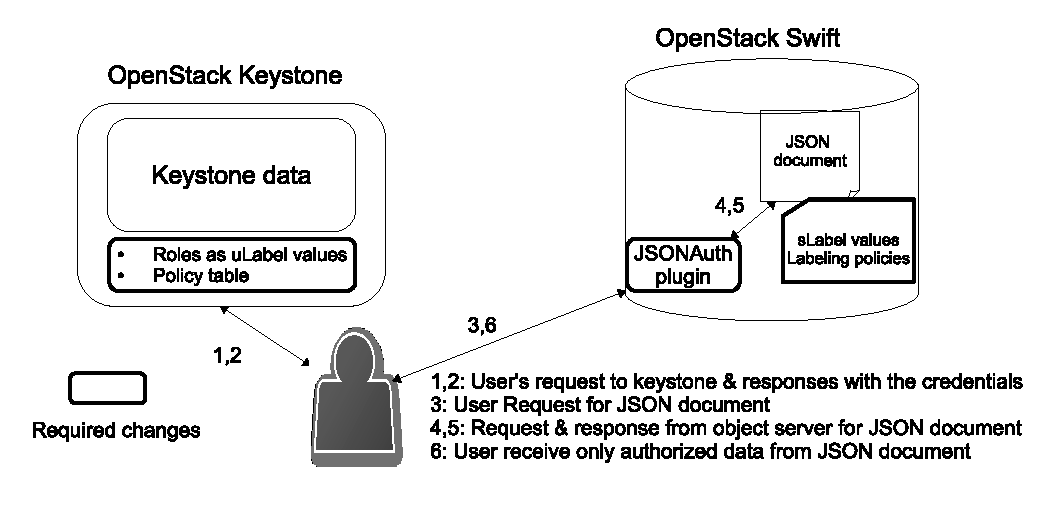
\includegraphics[width=.9\textwidth]{NSS16/implementation-in-swift}
 		\caption{Implementation in OpenStack IaaS cloud platform}
 		\label{fig:implementation-in-swift}
 	\end{figure}
 

We have implemented our proposed operational model and path-based labeling scheme in OpenStack IaaS cloud platform using OpenStack Keystone as the authorization service provider and OpenStack Swift as the storage service provider. Our choice of OpenStack is motivated by its support for independent and inter-operable  services and a well defined RESTful API set.

We have modified OpenStack Keystone and Swift services to accommodate required changes. A reference architecture of our testbed is given in Figure \ref{fig:reference-implementation-architecture}. Details of the implementation is shown in Figure \ref{fig:implementation-in-swift}. Required changes are presented as highlighted rectangles in Figure \ref{fig:implementation-in-swift}.

\subsection{Changes in OpenStack Keystone}

 OpenStack Keystone uses roles and role-based policies to provide authorization decisions. In our implementation, we uses roles to hold user-label attribute values. A set of valid security-label values are also stored as part of the Keystone service.
 
 Among two different types of policies - authorization and labeling policies, the former is managed in the Keystone service. We assume, a higher level administrators (possibly at the level of organization) adds, removes or updates these authorization policies. We add a policy table in Keystone database to store these enumerated authorization policies. 

\subsection{Changes in OpenStack Swift}

In Swift side, we store \textit{security-label} values assigned to JSON objects and path-based labeling policies applied to them.  Security-label values and labeling policies are stored as metadata of the stored objects, JSON documents in this case. For simplicity, we assume object owner (Swift account holder in this case) can update security-label values or labeling policies for stored JSON document. 


 During evaluation, we intercept every requests to Swift (from the Swift-proxy server) and reroute a request to be passed through \textit{JSONAuth plugin} if it is a request for a JSON document. In this case, the request additionally carries a requested path and authorization policies applicable to the user. JSONAuth plug-in retrieves the requested JSON document, apply path-based labeling policies to annotate the document and uses authorization policies to determine if the user is authorized for the requested content of the file. 

\subsection{Evaluation}

 \begin{figure} [t]
 	\centering
 	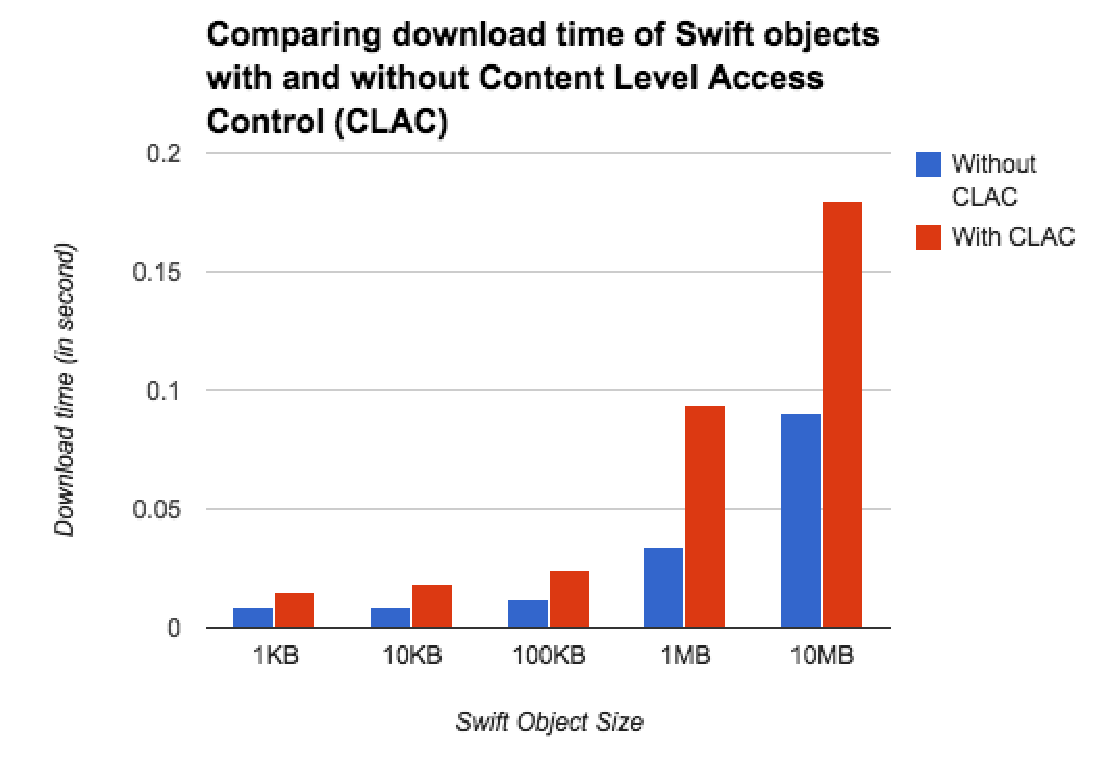
\includegraphics[width=.9\textwidth]{NSS16/performance}
 	\caption{Performance evaluation}
 	\label{fig:performance-a}
 \end{figure}


An evaluation of our implementation is shown in Figure \ref{fig:performance}. The evaluation has been made against concurrent download requests to the Swift proxy server. The X-axis shows size of the JSON document requested for download while the Y-axis shows the average download time for 10 concurrent request. Our evaluation shows a performance hit of nearly 60\% over no authorization protection.
%\textbf{Performance}



\section{Conclusion}
\label{sec:conclusion}
%Logical-formulas and enumerated  tuples are two major ways to specify authorization policies in an ABAC model.  In this paper, we show that they are equivalent in theoretical expressive power. We also analyze these models beyond their expressive power. We show that logical-formulas are flexible and convenient for setting up new authorization  policies but they are difficult to update/administer policies. On the other hand, enumerated authorization policies can be difficult to set up by enumerating all possible tuples but they are convenient for policy update and administration. We further show usefulness of enumerated policies by demonstrating how it supports micro policies and how it can be extended to be represented in a canonical form. 

In this paper, we present a finite attribute finite domain ABAC model using enumerated authorization policies. We then compare enumerated authorization policy ABAC models (\EPModels) with logical-formula authorization policy ABAC (\LPModels) models in finite domain. We show that they are equivalent in term of theoretical expressive power. We also analyze these models beyond their expressive power. While, logical-formulas are flexible and convenient for setting up new authorization  policies, enumeration is convenient for updating or administering policies. We also show that enumerated authorization policies facilitate micro-policies and can easily be represented in a canonical form. Canonical representation and support for micro policies enable automated and scalable administration. 

%Micro policies along with its canonical representation can help in automated and scalable administration. 

%A natural question to ask how we can take advantage of both approaches so that both specification of new policies and administration of existing policies are convenient. Can we combine enumerated and logical formula policies? Can we canonicalize logical formulas and take advantage in policy administration? Further research is also required to better understand micro policies and canonicalization of authorization policies. 

%* Connect with Ninguili's ARBAC evaluation perspectives.
\section{Acknowledgment}
This research is supported by NSF Grant CNS-1111925 and CNS-1423481.

\bibliographystyle{abbrv}
\bibliography{sigproc}
%\clearpage
%\appendix
%Appendix A

	 
%\balancecolumns % GM June 2007
% That's all folks!



%


%\subsection{Functional Specification}
\label{sec:session-management}
\begin{table*}
\centering
\caption{User-level session functions in \clabac{}}
\label{tab:session-management}
\begin{tabular}{|l|l|l|}
	\hline
\textbf{Fuction}                                                              & \textbf{Condition} & \textbf{Updates} \\ \hline

%\begin{tabular}[c]{@{}l@{}}\createSession\\ (u:U, s:S, values)\end{tabular} & \begin{tabular}[c]{@{}l@{}} $u \in U \land s \not \in S \land values \subseteq \uLabel(u) \setminus \{\createReq, \removeReq\}\  $ \\ $\createReq \in \uLabel(u) \land $ \\ $\exists\Policy_{\createSession} \equiv \{(\createReq, \sessionOL) \}\in \Policy$ \\ \end{tabular} &  \begin{tabular}[c]{@{}l@{}}$S' = S \cup \{s\}$ \\ $\creator(s) = u \land \sessionLabels(s)=value $ \end{tabular} \\\hline
%\multicolumn{3}{c}{\textbf{\textit{User level functions}}}\\ \hline

\begin{tabular}[c]{@{}l@{}}$\createSession$\\ $(u:U, s:S, values:2^{UL}$)\end{tabular} & \begin{tabular}[c]{@{}l@{}} $u \in U \land s \not \in S \land values \subseteq \uLabel(u)$  \end{tabular} &  \begin{tabular}[c]{@{}l@{}}$S' = S \cup \{s\}$,\\  $\creator(s) = u ,$ \\ $ \sessionLabels(s)=values $ \end{tabular} \\\hline


\begin{tabular}[c]{@{}l@{}}$\deleteSession$\\ $(u:U, s:S)$\end{tabular}   & \begin{tabular}[c]{@{}l@{}} $u \in U \land s  \in S \land creator(s)=u  $ \end{tabular}                   & \begin{tabular}[c]{@{}l@{}}$S' = S \setminus \{s\}$ \end{tabular}                             \\\hline


\begin{tabular}[c]{@{}l@{}}$\assignValues$\\ $(u:U,s:S, values:2^{UL}$)\end{tabular} &  \begin{tabular}[c]{@{}l@{}} $u \in U \land s  \in S \land creator(s)=u \ \land$ \\ $values \subseteq \uLabel(u)$ \end{tabular} &   \begin{tabular}[c]{@{}l@{}} $\sessionLabels(s)= \sessionLabels(s)$ \\ $\cup \ values $ \end{tabular}                \\ \hline


\begin{tabular}[c]{@{}l@{}}$\removeValues$\\ $(u:U,s:S, values:2^{UL}$)\end{tabular} &  \begin{tabular}[c]{@{}l@{}} $u \in U \land s  \in S \land creator(s)=u \ \land$  \\ $values \subseteq \uLabel(u)$ \end{tabular} &   \begin{tabular}[c]{@{}l@{}} $\sessionLabels(s)= \sessionLabels(s)$ \\ $\setminus \ values $ \end{tabular}                \\ \hline


\end{tabular}
\end{table*}



\eapABAC{} allows users to create or destroy sessions, and assign/remove values from an existing session. Table \ref{tab:session-management} presents user-level \textit{\sessionLabels{}} functions for managing sessions in \clabac{}. Each function is presented with formal parameters (given in the first column), necessary preconditions (in the second column) and resulting updates (in the third column).  The function $\createSession()$ creates a new session with given values, $\deleteSession()$ deletes an existing session, $\assignValues()$ assigns values in an existing session, and $\removeValues()$ removes values from an existing session. 

%First column in the table shows function names along with formal parameters, second column defines precondition which must be satisfied for the function to be executed. The third column describes updates in the LaBAC sets and relations once corresponding function is executed.

In \hlabac{}, we modify condition of the session functions from Table \ref{tab:session-management} to accommodate  that in a session created by a user, he can choose from the values he is assigned to or junior values. The modified conditions are given in Table \ref{tab:session-in-hlabac}. We specify an additional condition with each session function  in \consLabac{} and \labacOneOneOne{}.  For example, with $\createSession()$,  we specify a boolean function $f_{\createSession}()$ as additional precondition which must also be true. The definition of these boolean functions are  open-ended to be able to configure any session constraints. The difference between session functions in \consLabac{} and \labacOneOneOne{} is that the former does not consider hierarchy on user-label values whereas the later does. Table \ref{tab:session-in-consLabac} and \ref{tab:session-in-labacOne} show session functions in \consLabac{} and \labacOneOneOne{} respectively. Table \ref{tab:example-f-create-session} presents some examples of constraints specified with $f_{\createSession}()$ function.  \textit{Example 1} uses an enumerated policy, $\Policy_{\createSession}$. It specifies that in order to create a session and assign values to the session, a user must be assigned to value $\createReq$. \textit{Example 2} enforces the constraint that no more than one conflicting $\uLabel$ values can be activated in a session. \textit{Example 3} imposes that a user cannot have more than some bounded number of sessions.

Note that creation and deletion of objects, updating object-label values by sessions are outside the scope of \eapABAC{} operational models presented here. One reason behind is that, \eapABAC{} only focuses on attributes. It can be extended to include object creation and modification along the line of $ABAC_{\alpha}$ \cite{abacAlpha}. See Table \ref{tab:lbac-in-labac} for example.

\begin{table} 
\centering
 \captionsetup{justification=centering}
\caption{Session functions in \hlabac{} \newline (condition of session functions modified from Table \ref{tab:session-management} ) }
\label{tab:session-in-hlabac}
\begin{tabular}{|l|l|} \hline
\textbf{Function} & \textbf{Modified condition} \\ \hline
  $\createSession{}$      & \begin{tabular}[c]{@{}l@{}}  $u \in U \land s \not \in S \land values \subseteq$ \\ \hfill$  \{ ul' | \exists ul \udominate ul' [ ul \in \uLabel(u)] \}$ \end{tabular}             \\ \hline
	$\deleteSession{} $        & $u \in U \land s  \in S \land creator(s)=u  $                     \\ \hline
     $\assignValues{}$    &     \begin{tabular}[c]{@{}l@{}}  $u \in U \land s  \in S \land creator(s)=u \land values $ \\ \hfill$  \subseteq \{ ul' | \exists ul \udominate ul' [ ul \in \uLabel(u)] \}$ \end{tabular}                \\ \hline
 $\removeValues{}$    &     \begin{tabular}[c]{@{}l@{}}  $u \in U \land s  \in S \land creator(s)=u  \land values $ \\ \hfill$  \subseteq \{ ul' | \exists ul \in  \uLabel(u) \land ul \udominate ul' \}$ \end{tabular}                 \\ \hline
\end{tabular}
\end{table}



\begin{table}[]
\centering
 \captionsetup{justification=centering}
\caption{Session functions in  \consLabac{} (condition added with session functions from Table \ref{tab:session-management})}
\label{tab:session-in-consLabac}
\begin{tabular}{|l|l|} \hline
\textbf{Session function} & \textbf{Additional condition} \\ \hline
   $\createSession{}$      & $\land f_{\createSession}(u,s,values)$               \\ \hline
	$\deleteSession{} $        & $\land f_{\deleteSession}(u,s)$                     \\ \hline
     $\assignValues{}$    &      $\land f_{\assignValues}(u,s,values)$                \\ \hline
 $\removeValues{}$    &      $\land f_{\removeValues}(u,s,values)$                \\ \hline
\end{tabular}
\end{table}

\begin{table}[]
\centering
 \captionsetup{justification=centering}
\caption{Session functions in  \labacOneOneOne{} (condition added with session functions from Table \ref{tab:session-in-hlabac})}
\label{tab:session-in-labacOne}
\begin{tabular}{|l|l|} \hline
\textbf{Session function} & \textbf{Additional condition} \\ \hline
   $\createSession{}$      & $\land f_{\createSession}(u,s,values)$               \\ \hline
	$\deleteSession{} $        & $\land f_{\deleteSession}(u,s)$                     \\ \hline
     $\assignValues{}$    &      $\land f_{\assignValues}(u,s,values)$                \\ \hline
 $\removeValues{}$    &      $\land f_{\removeValues}(u,s,values)$                \\ \hline
\end{tabular}
\end{table}



\begin{table}
	\centering
 \caption{Examples of $f_{\createSession}(u, s, values)$}
 \label{tab:example-f-create-session}
	\begin{tabular}{|l|}
		\hline	                                                                                           	
		%\multicolumn{1}{|c|}{\underline{\textit{Examples in \consLabac{}/\labacOneOneOne{}:}}}\\                	
		\multicolumn{1}{|l|}{{\textit{Example 1. using \eapABAC{} policy:}}}\\
		
		$\exists \createReq \in \uLabel(u) \land$ \\$ \exists \Policy_{\createSession} \equiv \{(\createReq, \sessionOL) \}\in \Policy$ \\
		
		\\ \multicolumn{1}{|l|}{{\textit{Example 2. using \labacOneOneOne{} session constraint CSL:}}}\\
		 $|values \cap OneElement(CSL)| \le 1$ \\
		 
		 \\\multicolumn{1}{|l|}{{\textit{Example 3. using cardinality  constraint on sessions:}}}\\
		 $|\{s | \creator(s)=u\}| \le 10$ \\
		 \hline
		\end{tabular}  

\end{table}


\end{document}
